\documentclass[12pt, oneside, titlepage]{article}   	% use "amsart" instead of "article" for AMSLaTeX format

\usepackage{graphicx}
\graphicspath{ {\string} }
\usepackage{subcaption}

%%%%%%%%%%%%%%%%%%%%%%%%%%%%%%%%%%%%%%%%%%%%%%%%%%%%
% set up packages
%%%%%%%%%%%%%%%%%%%%%%%%%%%%%%%%%%%%%%%%%%%%%%%%%%%%
\usepackage{geometry}                
\usepackage{textcomp}                
\usepackage{amsmath}                
\usepackage{graphicx}                
\usepackage{amssymb}                
\usepackage{fancyhdr}                
\usepackage{subcaption}                
\usepackage{bm}                
\usepackage{tabularx}                

\usepackage{lineno}
% package for comments
\usepackage{soul}

\usepackage[breaklinks=true]{hyperref}

\usepackage[superscript,noadjust]{cite} % puts dash in citations to abbreviate
\usepackage [autostyle, english = american]{csquotes} % sets US-style quotes

\usepackage{etoolbox} % block quotes

\usepackage{float}
\usepackage{color}

\usepackage{pgf}
\usepackage{tikz}
\usepackage{eqnarray}

\usepackage{listings} % code blocks
\usepackage{setspace}

\usepackage{lscape}

% tikz background
\usetikzlibrary{backgrounds, fit}


\usepackage{natbib}
%\bibliographystyle{abbrvnat}
\setcitestyle{authoryear,open={(},close={)}}

%%%%%%%%%%%%%%%%%%%%%%%%%%%%%%%%%%%%%%%%%%%%%%%%%%%%
% call packages
%%%%%%%%%%%%%%%%%%%%%%%%%%%%%%%%%%%%%%%%%%%%%%%%%%%%	
\geometry{letterpaper, marginparwidth=60pt} % sets up geometry              		
\linenumbers % adds line numbers 
\MakeOuterQuote{"} % sets quote style
\doublespacing % setspace

%%%%%%%%%%%%%%%%%%%%%%%%%%%%%%%%%%%%%%%%%%%%%%%%%%%%
% patches with etoolbox 
%%%%%%%%%%%%%%%%%%%%%%%%%%%%%%%%%%%%%%%%%%%%%%%%%%%%	
% block quotes
\AtBeginEnvironment{quote}{\small}

% linenumbers
\makeatletter
\patchcmd{\@startsection}{\@ifstar}{\nolinenumbers\@ifstar}{}{}
\patchcmd{\@xsect}{\ignorespaces}{\linenumbers\ignorespaces}{}{}
\makeatother

%%%%%%%%%%%%%%%%%%%%%%%%%%%%%%%%%%%%%%%%%%%%%%%%%%%%
% tikzlibrary modifications
%%%%%%%%%%%%%%%%%%%%%%%%%%%%%%%%%%%%%%%%%%%%%%%%%%%%	
\usetikzlibrary{fit}
\usetikzlibrary{positioning}
\usetikzlibrary{arrows}
\usetikzlibrary{automata}
\usetikzlibrary{shapes.misc}

% https://tex.stackexchange.com/questions/118223/drawing-little-semicircle-to-show-that-two-intersecting-lines-are-not-connected
\usetikzlibrary{calc}

% \intersect{<p1>}{<p2>}{<q1>}{<q2>}
% draws the line p1--p2, showing a little semicircle
% where it intersects the line q1--q2.
\newcommand\intersect[4]{
  \draw let \p{c} = (intersection of #1--#2 and #3--#4) in
    (#1) -- ($(\p{c})!0.75mm!(#1)$) 
    to[bend right=90] ($(\p{c})!0.75mm!(#2)$) -- (#2)
}



%%%%%%%%%%%%%%%%%%%%%%%%%%%%%%%%%%%%%%%%%%%%%%%%%%%%
% page formatting; exact 1 in margins
%%%%%%%%%%%%%%%%%%%%%%%%%%%%%%%%%%%%%%%%%%%%%%%%%%%%
\pagestyle{plain}                                                     

\setlength{\textwidth}{6.5in}    
\setlength{\oddsidemargin}{0in}
\setlength{\evensidemargin}{0in}
\setlength{\textheight}{8.5in}
\setlength{\topmargin}{0in}
\setlength{\headheight}{0in}
\setlength{\headsep}{0in}
\setlength{\footskip}{.5in}

%%%%%%%%%%%%%%%%%%%%%%%%%%%%%%%%%%%%%%%%%%%%%%%%%%%%
% defining code blocks using listings package
%%%%%%%%%%%%%%%%%%%%%%%%%%%%%%%%%%%%%%%%%%%%%%%%%%%%

\definecolor{dkgreen}{rgb}{0,0.6,0}
\definecolor{gray}{rgb}{0.5,0.5,0.5}
\definecolor{mauve}{rgb}{0.58,0,0.82}

\lstset{frame=tb,
  language=R,
  aboveskip=3mm,
  belowskip=3mm,
  showstringspaces=false,
  columns=flexible,
  basicstyle={\small\ttfamily},
  numbers=none,
  numberstyle=\tiny\color{gray},
 % keywordstyle=\color{blue},
  commentstyle=\color{dkgreen},
  stringstyle=\color{mauve},
  breaklines=true,
  breakatwhitespace=true,
  tabsize=3,
  otherkeywords={0,1,2,3,4,5,6,7,8,9},
  deletekeywords={data,frame,length,as,character,dunif,ps},
}

%%%%%%%%%%%%%%%%%%%%%%%%%%%%%%%%%%%%%%%%%%%%%%%%%%%%
%%%%%%%%%%%%%%%%%%%%%%%%%%%%%%%%%%%%%%%%%%%%%%%%%%%%
% begin document
%%%%%%%%%%%%%%%%%%%%%%%%%%%%%%%%%%%%%%%%%%%%%%%%%%%%
%%%%%%%%%%%%%%%%%%%%%%%%%%%%%%%%%%%%%%%%%%%%%%%%%%%%

\begin{document}

Last updated: \today

\section{Introduction}

\hl{Introduction} Soil seed banks can be a key part of plant life history strategies that rely on bet hedging and predictive germination to persist in variable environments. Theory and empirical work on seed banks have a long history. Integrating this knowledge into demographic models has proven more challenging. While aboveground individuals can be readily observed, additional experiments are often required to estimate seed survival, viability, and germination. Studies have identified consequences to omitting seed banks from stage-structured models and highlighted the effects of parameter uncertainty associated with dormant stages.

\hl{Conservation implications} Seed banks are generally important for persistence and potentially critical for rare/endangered plant species. Selecting seeds with seed banks can be an important part of restoration strategies \hl{Barga and Leger}. Persistent seed banks may be critical for helping species make it through periods of environmental uncertainty, for desiccation resistant seeds in arid climates experiencing droughts as well as for seeds that must remain moist in tropical climates. 

\hl{Seed banks in structured models: matrix structure} Structured demographic models (whether matrix models or integral projection models) require choices about the structure of the life cycle. It's possible to evaluate the consequences of incorrectly specifying the life cycle by, for example, omitting the seed bank stage when it is important. For example, \cite{doak2002,nguyen2019} reviewed published seed bank studies and assessed the effects of removing seed banks on the estimated population growth rate. 

\hl{Seed banks in structured models: parameter uncertainty} Parameter uncertainty can also influence estimates of population growth rate. Because relatively little is often known about the seed bank, authors may be less likely to include uncertainty in their assumptions. \cite{paniw2017} evaluated the consequences of uncertainty associated with seed bank transitions and quantified the effect of this uncertainty on estimates of population growth rate and population extinction. So, we know that it can be important to include seed banks and that uncertainty about them can be important.

\hl{Seed banks in structured models: data-parameter mismatch} One challenge is that we are often interested in conditional probabilities; say, the probability of survival or germination for a 2-year old seed. However, because seeds are buried in the soil we can not observe the events leading up to a particular outcome. This idea is closely related to the concept of a hazard in survival analysis \hl{Zens and Peart 2003}, also referred to as the 'force of mortality'. This reflects the instantaneous death rate. While we may want to observe how this changes over time, we often only have data from the end of a time period. 

\hl{Focus of this article: new models, model checking} An important gap is that there seem to be few ways of checking whether particular representations of seed bank persistence are appropriate. Building a model checking and/or model selection step into the process of constructing stage-structured population models creates the opportunity to consider a richer array of data when modeling seed bank. For example, \cite{peterson2019} describe model selection for considering beta vs. normal growth.

\hl{Motivation: Clarkia} We encountered these challenges when we sought to estimate seed survival and germination for population models of the winter annual Clarkia xantiana ssp. xantiana. We thus built on existing approaches by developing and evaluating a hierarchical model that includes a process component to represent loss from the seed bank via decay and germination, and a sampling model to represent the design of the seed burial experiments. Finally, we combined data from estimates of reproduction and seedling emergence in permanent plots with the seed experiments. We used our approach to assess the extent of intraspecific variation in the seed survivorship curve and in age-specific germination for seeds of C. xantiana.

We observed substantial variation in the survivorship curves of seeds in our C. xantiana study populations, corresponding to Type I, II, and III seed survivorship trajectories. The Weibull survival process proved to be a good representation of persistence in the seed bank, and population-level estimates for the shape parameter ranged from .25 to 1.25. We summarized uncertainty about the full survivorship curve as a function of both the shape and inverse-rate parameter. We also propagated uncertainty about survival to estimates of age-specific germination.

In addition to fitting our model to empirical data, we conducted a simulation study to aid with computational implementation. We compared a nonparametric representation of seed survival and several parametric survival functions (negative exponential, continuous exponential, Weibull). We simulated data from each survival process and fit models to confirm we recovered known parameter combinations. We also tested the consequences of fitting a model to data generated under a different process (e.g. fit a model with nonparametric survival to data generated by a Weibull). Overall, we propose that one of the strengths of the approach we describe is that it makes it possible to compare representations of seed decay and germination in the model fitting step before moving on to evaluating its impact on population growth rate. 

\hl{Goals} Our approach to analyzing seed bag burial experiments contributes to efforts to make richer inferences from the trove of demographic data collected by plant ecologists. The combination of data from aboveground observations and belowground experiments highlights the value of data fusion techniques even in the case of relatively small datasets. (1) Survey combination of data collection and modeling approaches for seed banks. (2) Describe continuous representations of seed survival in the soil seed bank. (3) Use product integral to combine processes of germination and seed survival. (4) Highlight careful model selection as tool to supplement construction of structured models with seed banks.

\hl{Outline} (Aim 1) Explain product integral and P(S)*P(G) (Aim 2) Describe approach for the simplest case: exponential model, constant germination, ie. unstructured seed bank. Simulate for different values of decay and germination, attempt to recover parameters. Plot 1: show 'true' decay+germination, simulated values, and estimated decay+germination. Plot 2: repeat for a range of k+germination values, from low-high half-life (0-1) to show that sampling variance is highest in the middle, and that uncertainty in parameter estimates can increase at old ages even in unstructured model. Plot 3: true vs. observed parameter values for different sample sizes. (Aim 3) Introduce Weibull model and explain why alternative decay functions might be of interest. Repeat simulations from Aim 2 but only show Plot 2+Plot 3.


\section{Literature review}

To examine the range of strategies used to model seed banks, we examined data associated with COMPADRE. We identified all matrix models that included seeds or seed banks, and read the associated publications to identify how the authors handled seed stages. Before reading papers for this project, we developed a preliminary coding scheme based on our general understanding of methods in the literature. We considered the following categories for data collection: (1) no data, (2) lab experiments, (3) field experiments, (4) observations, (5) combination. We considered the following categories for representation in models: (1) ignore seed bank, (2) model rates as constant, (3) model rates as random, (4) model rates as function of covariates, (5) model rates with differential equations.

We applied our coding scheme to the literature and then discussed the codings to refine our callings. We summarize our findings in a table (supplement) and in a matrix that cross-tabulates data collection and model representation to understand how ecologists implement methods to study seed banks.

\singlespace
\begin{itemize}

\item \hl{Fox 2001; Failure time analysis chapter}, \hl{Zens and Peart 2003}

\item \hl{McNair, Seed Science Research 2012}. Discuss non-parametric and semi-parametric methods for seed germination data.

\item \hl{Paniw et al. 2016} describe the consequences of parameter uncertainty in dormant life stages on stochastic demographic models.

\item \hl{Meyer et al. 2006} 12 year seed bank experiment with Lepidium

\item \hl{Menges 2000} reviews plant PVAs

\item \hl{Satterthwaite et al. 2007} conservation application

\item \hl{Peterson et al. 2019} discusses improving structured models with representations of non-normal growth; similar logic could be applied to seed bank.

\item \hl{Bartholomew et al. 1973} and \hl{Lewis 1962} discuss catastrophic selection and lack of seed bank in Clarkia. 

\item \hl{Ecology of Soil Seed Banks}: book describing the soil seed bank, includes chapter by Venable on evolutionary ecology.

\item \hl{Doak et al. 2002} describes challenges of modeling seed banks

\end{itemize}
\doublespace

\section{Models}

Seed banks present a challenge for models of plant population demography. Individual seeds can not be tracked in the field so ecologists have turned to various methods to assess survival and germination from the seed bank, including experimental burials and seed addition experiments. This makes seed banks a good case for combining observation and process models in order to separate variation due to sampling and variation due to the process in question. 


While inputs to the soil seed bank come solely from seed rain, seeds can leave the soil seed bank through various routes. These may include predation, pathogens, deep burial, physiological death, failed germination, and successful germination \hl{Simpson et al. Ch. 1 Ecology of seed banks; Figure 1}. Seeds can be destroyed by predators or decomposers, lose viability through natural causes (i.e. age-related loss of vitality) \hl{Baker Chapter 2 Ecology of seed banks}

See \hl{Baskin and Baskin Chapter X Ecology of seed banks} for description of progression of dormancy. See \hl{McCue and Holtsford 1998} for description of how dormancy progresses over time in Clarkia.

Seeds leave the soil seed bank through destruction, physiological death, and germination. The persistence of seeds in the soil combines discrete and continuous processes. Seeds leave the seed bank through germination (discrete) or destruction (continuous). The persistence of seeds to the first winter combines destruction and physiological death. However, in January we only directly observe seed loss due to destruction. We also observe loss through germination. Seeds are then buried again and unearthed in October at which point we observe additional loss due to destruction. We also estimate physiological death at that time. We estimate loss due to destruction at January. We estimate loss due to germination at January. We then estimate loss due to destruction in October, conditional on not being destroyed or germinating in January. Finally, we then estimate loss due to physiological death in October, conditional on not being destroyed. We want to estimate the loss due to physiological death, conditional on not germinating and not being destroyed in January;

Loss of seeds from the soil seed bank reflect the product of destruction and germination. Seeds that persist to a given time are those that have not been destroyed and did not germinate. Additionally, we estimate the proportion of seeds that persist to October of each year that are viable. However, these tests are conducted on a subset of seeds; we can say viability in October | intact in October. We are interested in the proportion of seeds that did not germinate and are intact in January that are viable. To get this number requires some additional assumptions. The product of persistence and viability gives the expected proportion of seeds viable in October. 

Here is another option. I could estimate viability in October and then calculate the proportion of seeds that are viable in January using either an exponential decay OR assuming decay proceeds at the same rate as physical death. In either case, we just use data from each age to estimate the viability of seeds of that age, rather than inferring the viability of seeds at all points in time. 

Basically, describe two different events (physical destruction) and (germination). The curve for physical destruction is the product of seed decay and germination. Germination is discrete and includes survival to time x, viability at time x, and then germination. 

The persistence of seeds beyond the first germination time is thus conditional on the absence of germination. Both germination and mortality remove seeds from the soil seed bank; we define hazard functions for these events. The survival function thus describes the persistence of seeds in the soil (seeds that do not experience mortality or germination).

The survival function is defined by the product integral of the discrete and continuous hazards:
%
\begin{align}
  \begin{split}
\Pr( B|A )  & = \frac{\Pr( A|B ) \Pr( B )}{ \Pr ( A )} \\
\Pr( g | s )  & = \frac{\Pr( s | g ) \Pr( g )}{ \Pr ( s )} \\ 
 \Pr( g ) & = Pr( g | s ) \Pr( s ) \
  \end{split}
\end{align}
%

Finally, seeds can also leave the soil seed bank through loss of viability. We expect that loss of viability is a continuous process but our estimates of viability are discrete.

 For the deterministic process model, I turned to literature on litter decomposition \hl{e.g. Olson 1963, Cornwell et al. 2014}. \hl{Cornwell et al. 2014} describe several functions that I considered as "process models". Some of these are the same as the survival functions underlying the models in \hl{Rees and Long 1993}. There are several models that could be considered to represent the survival process that I briefly describe below. A separate study with different objectives might be interested in coding up these competing models and using model selection to evaluate the relative support for different models of survival. 

The negative exponential model corresponds to a constant decay rate, as in \hl{Gremer and Venable 2014}. This model has a constant decay parameter $k$ that implies the decaying material be treated as a homogeneous mass with each seed having an equal probability of mortality throughout time. The negative exponential decay model may be appropriate if seed survival is random in time and largely unrelated to seed characteristics. But we know that seeds exhibit phenotypic variation in dormancy-related traits \hl{Lonsdale 1988}.

The continuous exponential model is one in which seed mortality is described by a continuous quality distribution. For example, if seed survival is a function of a continuous phenotypic trait, we could imagine this model describing the survival process. 

The Weibull residence time model represents the seed pool as a distribution of survival times. Parameter alpha controls the shape of the decomposition trajectory and beta the rate of decomposition. This model can reduce to the exponential model when alpha is 1. If alpha is less than 1, the decomposition rate decreases through time. If alpha is greater than 1, the decomposition rate increases through time. 

The table below summarizes the models we considered, the parameters, and the number of parameters for each model. The product of the mortality and germination process is a deterministic function that equals the average proportion of seeds that are expected to be intact or germinated. This average proportion is the mean of a beta distribution with process variance that captures variation beyond the effect of seed age on mortality as represented with a mortality process and germination.  We might also consider a germination process where germination is randomly distributed and independent for each bag?

\singlespace

\begin{center}
\captionof{table}{ Deterministic process models for seed mortality and germination } \label{tab:title2} 
 \begin{tabularx}{\linewidth}{l c c c c} 
 \hline
 \hline
 \multicolumn{1}{ c }{ Model } & 
\multicolumn{1}{ c }{ Mortality process } & 
\multicolumn{1}{ c }{ Germination process } & 
 \multicolumn{1}{ c }{ Parameters } & 
  \multicolumn{1}{ c }{ Parameter number }   \\
 \hline
 %%%% VIABILITY TRIALS
% \multicolumn{2}{ l }{ \sc{Viability trials }} \\

 A1 & Negative exponential & Constant & $k,g$ & 2 \\

 A2 & Negative exponential & Age-dependent & $k,g_{1-3}$ & 4 \\
 
  B1 &  Compound exponential & Constant & $a,b,g$ & 3  \\

  B2 &  Compound exponential & Age-dependent & $a,b,g_{1-3}$ & 5\\

  C1 &   Weibull residence time & Constant & $\alpha,\beta,g$ & 3 \\

  C2 &   Weibull residence time & Age-dependent & $\alpha,\beta,g_{1-3}$ & 5 \\
  
  \hline
\end{tabularx}
\end{center}

\doublespace



\subsection{Linking to seed pots}

The seed bag burial experiment made it possible to estimate conditional germination; that is, the probability of germination for seeds of a given age that were intact at a given time. In the seed pot experiment, observations of seedlings reflect unconditional germination; the probability of emergence for a seedling that was buried some time ago. This process reflects both seed survival and conditional germination, but we only observe the emergence outcome.

In the model defined above, survival has been reduced to a two-parameter process: roughly, a scale and shape parameter. I estimated a population-level shape parameter ($\alpha_j$) that defines how the probability of survival changes through time. For each population, I estimated a scale parameter ($\eta_{jk}$) for each year; this describes the magnitude of change and essentially shifts the survival curve up or down. The posteriors from these estimates could serve as informed priors.

For the seed pot data, we only have observations on unconditional germination. The latent probability would thus be the product of survival up to the time of germination and conditional germination. This amounts to changing the equations for the compound event histories to reflect the events under observation. The germination probabilities are indexed by site $j$, experimental year $k$, and age $l$; for example, emergence of 1-year old seeds at site $j$ from the experimental year $k$ is given by $\gamma_{jkl}$. The compound event histories are now defined as:
\singlespace
%
\begin{align}
  \begin{split}
\theta_{j1,1} & = \gamma_{j1,1} \\
\theta_{j1,2} & = (1-\gamma_{j1,1}) \times \gamma_{j1,2} \\
\theta_{j1,3} & = (1-\gamma_{j1,1}) \times (1-\gamma_{j1,2}) \gamma_{j1,3} \\
  \end{split}
\end{align}
%
\doublespace
In each experimental year $k$, we have data on emergence 1, 2, and 3 years after the seeds were buried. Multiplying these with the survival functions returns the unconditional probability of germination, which is the latent probability underlying the binomial likelihood for the observed counts of seedlings.

We would use the estimates for the parameters of the survival functions from the seed bags as informed priors. The posteriors on parameters of the survival function would remain the same if the data from the seed pot experiments was consistent with the estimates from after the seed bag experiments. They would change if additional information from the seed pot experiments influenced the estimate. Similarly, the population-level conditional germination probabilities could also serve as informed priors. 

\subsection{Model selection}

For the deterministic process model, I turned to literature on litter decomposition \hl{e.g. Olson 1963, Cornwell et al. 2014}. \hl{Cornwell et al. 2014} describe several functions that I considered as "process models". Some of these are the same as the survival functions underlying the models in \hl{Rees and Long 1993}. There are several models that could be considered to represent the survival process that I briefly describe below. A separate study with different objectives might be interested in coding up these competing models and using model selection to evaluate the relative support for different models of survival. 



\section{Overview}

Seed banks present a challenge for models of plant population demography. Individual seeds can not be tracked so ecologists have turned to various methods to assess survival and germination from the seed bank, including experimental burials and seed addition experiments. The base assumption is often that seed mortality proceeds at a constant rate. Although this assumption has repeatedly been challenged \hl{Lonsdale 1988, Rees and Long 1993} there remain limited assessments for how appropriate it is. 

One challenge is that we are often interested in conditional probabilities; say, the probability of survival or germination for a 2-year old seed. However, because seeds are buried in the soil we can not observe the events leading up to a particular outcome. This idea is closely related to the concept of a hazard in survival analysis \hl{Zens and Peart 2003}, also referred to as the 'force of mortality'. This reflects the instantaneous death rate. While we may want to observe how this changes over time, we often only have data from the end of a time period. 

Conditional versus unconditional probability \hl{Christian and Stanton 2004}, \hl{Vitalis et al. 2004}, \hl{Rees and Long 1993}, \hl{Rees and Long 1992}, \hl{Kalisz 1991}, \hl{Templeton and Levin 1979}, \hl{Venable 1989}. Conditional probabilities of survival and germination are conditional on survival up to a point. 
%
\begin{align}
  \begin{split}
\Pr( B|A )  & = \frac{\Pr( A|B ) \Pr( B )}{ \Pr ( A )} \\
\Pr( g | s )  & = \frac{\Pr( s | g ) \Pr( g )}{ \Pr ( s )} \\ 
 \Pr( g ) & = Pr( g | s ) \Pr( s ) \
  \end{split}
\end{align}
%

Three works illustrate some of the range of approaches that have been used to study seed dynamics. \hl{Kalisz 1991} describes a seed burial experiment in which known numbers of seeds were buried and unearthed after varying periods of time. Kalisz estimates unconditional and conditional survival and emergence probabilities over the course of two years. \hl{Rees and Long 1993} present an analysis of experimental seed burials that focuses on seedling recruitment. They fit several distributions to 5 years of data on emerged seedlings, and use goodness-of-fit tests to assess the survival functions they consider. \hl{Gremer and Venable 2014} estimate seed survival by assuming a constant mortality rate throughout the year for new seeds and one-year old seeds (\hl{Gremer and Venable Appendix S1}). Their study uses estimates of seed production and soil cores to infer the rate of survival.

Our seed bag experiment combines some features of these studies. We used seed bags buried with known numbers of seeds to estimate seedling emergence and survival as a function of age in three consecutive years. We thus have data on unconditional survival and emergence probabilities. Sampling seed bags at the end of each experimental year was also destructive. And as is generally the case we do not have independent information about survivorship patterns in the seed bank that could inform whether or not seed mortality is constant.    

Here, I give a general overview of the approach we used to understand the dynamics of seeds. Although the full model is hierarchical, I ignore the hierarchical component in my explanation at this point. Because we have data on both seed survival and germination, we developed models that used both parts of the experiment. For seed bags that were unearthed in February, the field crew counted the germinants as well as the intact, ungerminated seeds. I used these counts to estimate the conditional probability of germination for 1-, 2-, or 3-year old seeds in each experimental round. 

The sum of counts of germinants and intact, ungerminated seeds in February of a given year correspond to the unconditional probability of surviving to that time. Likewise, the counts of intact seeds in October of a given year correspond to the unconditional probability of surviving to that time. If individual bags were followed over the course of the entire experiment, it might be possible to estimate the probability of survival between time points because it would be unlikely (or impossible) that bags would gain seeds over the course of the experiment. However, sampling in October of each experimental year was destructive and so seed counts increased between time points because of sampling variation. 

To represent the experimental design and model the survival process, I developed a model with a binomial likelihood (the sampling model) and a deterministic process model that represents survival. Because we don't know which model best represents the survival process in our seeds, I chose to work with the Weibull residence time model. The Weibull is a flexible model that can represent a range of decay/survival trajectories \hl{Cornwell et al. 2014}, is used in survival analysis \hl{Klein and Moeschberger 2003; Pinder et al. 1978}, and has been applied to other problems in ecology and evolutionary biology \hl{Smits 2015; Dahlgren et al. 2016}. Fitting a model with a Weibull survival process doesn't preclude the possibility that seed mortality is constant; the negative exponential model is a subset. 

Crucially, seeds in the seed bags are subject to these two separate processes: germination and survival. For example, to estimate the probability that a seed survives to October of year two, we need to account for both the probability that the seed remains intact (does not suffer mortality) and the probability that the seed does not germinate. I linked the germinant and seed counts to jointly estimate the survival and germination probability; the estimates of survival thus incorporate information about the probability of germination. 

Finally, seed production happens in June/July but the seed bags were buried in October. To estimate survival between seed production and the start of the seed bag experiment, I used estimates of seed production and seedling emergence in the permanent plots to \hl{Eckhart et al. 2011}. In two experimental years, we had data on the number of seeds entering a plot and the number of seeds emerging alongside the seed bag experiment. I summed counts across all plots and wrote an additional likelihood statement for the probability of observing those counts. The additional likelihood composed the unobserved probability of surviving from seed production to October with the probability of survival from October to February (given by the deterministic survival process) and the probability of germination. 

 For the deterministic process model, I turned to literature on litter decomposition \hl{e.g. Olson 1963, Cornwell et al. 2014}. \hl{Cornwell et al. 2014} describe several functions that I considered as "process models". Some of these are the same as the survival functions underlying the models in \hl{Rees and Long 1993}. There are several models that could be considered to represent the survival process that I briefly describe below. A separate study with different objectives might be interested in coding up these competing models and using model selection to evaluate the relative support for different models of survival. 

The negative exponential model corresponds to a constant decay rate, as in \hl{Gremer and Venable 2014}. This model has a constant decay parameter $k$ that implies the decaying material be treated as a homogeneous mass with each seed having an equal probability of mortality throughout time. The negative exponential decay model may be appropriate if seed survival is random in time and largely unrelated to seed characteristics. But we know that seeds exhibit phenotypic variation in dormancy-related traits (\cite{lonsdale1988}).

The continuous exponential model is one in which seed mortality is described by a continuous quality distribution. For example, if seed survival is a function of a continuous phenotypic trait, we could imagine this model describing the survival process. 

The Weibull residence time model represents the seed pool as a distribution of survival times. Parameter alpha controls the shape of the decomposition trajectory and beta the rate of decomposition. This model can reduce to the exponential model when alpha is 1. If alpha is less than 1, the decomposition rate decreases through time. If alpha is greater than 1, the decomposition rate increases through time. 

The table below summarizes the models we considered, the parameters, and the number of parameters for each model. The product of the mortality and germination process is a deterministic function that equals the average proportion of seeds that are expected to be intact or germinated. This average proportion is the mean of a beta distribution with process variance that captures variation beyond the effect of seed age on mortality as represented with a mortality process and germination.  We might also consider a germination process where germination is randomly distributed and independent for each bag?

\singlespace

\begin{center}
\captionof{table}{ Seed bag dataset models } \label{tab:title2} 
 \begin{tabularx}{\linewidth}{l c c c c} 
 \hline
 \hline
 \multicolumn{1}{ c }{ Model } & 
\multicolumn{1}{ c }{ Mortality process } & 
\multicolumn{1}{ c }{ Germination process } & 
 \multicolumn{1}{ c }{ Parameters } & 
  \multicolumn{1}{ c }{ Parameter number }   \\
 \hline
 %%%% VIABILITY TRIALS
% \multicolumn{2}{ l }{ \sc{Viability trials }} \\

 A1 & Negative exponential & Constant & $k,g$ & 2 \\

 A2 & Negative exponential & Age-dependent & $k,g_{1-3}$ & 4 \\
 
  B1 &  Compound exponential & Constant & $a,b,g$ & 3  \\

  B2 &  Compound exponential & Age-dependent & $a,b,g_{1-3}$ & 5\\

  C1 &   Weibull residence time & Constant & $\alpha,\beta,g$ & 3 \\

  C2 &   Weibull residence time & Age-dependent & $\alpha,\beta,g_{1-3}$ & 5 \\
  
  \hline
\end{tabularx}
\end{center}

\doublespace



The table above shows the survival, probability mass, and hazard functions for the persistence of seeds in the soil. It also shows the survival, probability mass, and hazard functions for viable seeds in the soil. 
Because the event $X$ here is the mortality of seeds, the probability of survival over an interval is the complementary probability to the hazard function. Seeds that physically persist in the soil may be physiologically dead, so this is closer to apparent survival as in the mark-recapture literature. The table above can be translated into parameters used in the stage-structured matrix model as follows:

\singlespace

\begin{center}
\captionof{table}{ Structured model parameters conditional on persistence only } \label{tab:title} 
 \begin{tabularx}{\linewidth}{c l c } 
 \hline
 \hline
  \multicolumn{1}{ c }{Matrix parameter} & 
  \multicolumn{1}{ c }{Probability statement } & 
   \multicolumn{1}{ c }{ Probability }  \\
   \hline
   
    $g_1$ & $P(G_1 | S_1)$ & $  \gamma_1  $ \\

 $g_2$ & $P(G_2 | S_3,S_2,G^c_1,S_1)$  & $  \gamma_2 $ \\

 $g_3$ &  $P(G_3 | S_5,S_4,G^c_2S_3,S_2,G^c_1,S_1)$ & $  \gamma_3 $ \\
 
 \hline

 $s_1$ & $P(S_1)$ & $ \theta_1$ \\

 $s_2$ &  $P(S_2|G^c_1,S_1)$ &  $ \theta_3 / \theta_2 $  \\

$s_3$ &   $P(S_3|S_2,G^c_1,S_1)$ & $ \theta_4 / \theta_3  $ \\
 
$s_4$ &   $P(S_4|G^c_2S_3,S_2,G^c_1,S_1)$ &  $  \theta_6 / \theta_5 $ \\
   
$s_5$ & $P(S_5|S_4,G^c_2S_3,S_2,G^c_1,S_1)$ &  $ \theta_7 / \theta_6  $  \\
 
 $s_6$ & $P(S_6|G^c_3,S_5,S_4,G^c_2S_3,S_2,G^c_1,S_1)$ &  $ \theta_9 / \theta_8  $  \\
 
  \hline
\end{tabularx}
\end{center}




While inputs to the soil seed bank come solely from seed rain, seeds can leave the soil seed bank through various routes. These may include predation, pathogens, deep burial, physiological death, failed germination, and successful germination \hl{Simpson et al. Ch. 1 Ecology of seed banks; Figure 1}. Seeds can be destroyed by predators or decomposers, lose viability through natural causes (i.e. age-related loss of vitality) \hl{Baker Chapter 2 Ecology of seed banks}

See \hl{Baskin and Baskin Chapter X Ecology of seed banks} for description of progression of dormancy. See \hl{McCue and Holtsford 1998} for description of how dormancy progresses over time in Clarkia.

Seeds leave the soil seed bank through destruction, physiological death, and germination. The persistence of seeds in the soil combines discrete and continuous processes. Seeds leave the seed bank through germination (discrete) or destruction (continuous). The persistence of seeds to the first winter combines destruction and physiological death. However, in January we only directly observe seed loss due to destruction. We also observe loss through germination. Seeds are then buried again and unearthed in October at which point we observe additional loss due to destruction. We also estimate physiological death at that time. We estimate loss due to destruction at January. We estimate loss due to germination at January. We then estimate loss due to destruction in October, conditional on not being destroyed or germinating in January. Finally, we then estimate loss due to physiological death in October, conditional on not being destroyed. We want to estimate the loss due to physiological death, conditional on not germinating and not being destroyed in January;

Loss of seeds from the soil seed bank reflect the product of destruction and germination. Seeds that persist to a given time are those that have not been destroyed and did not germinate. Additionally, we estimate the proportion of seeds that persist to October of each year that are viable. However, these tests are conducted on a subset of seeds; we can say viability in October | intact in October. We are interested in the proportion of seeds that did not germinate and are intact in January that are viable. To get this number requires some additional assumptions. The product of persistence and viability gives the expected proportion of seeds viable in October. 

Here is another option. I could estimate viability in October and then calculate the proportion of seeds that are viable in January using either an exponential decay OR assuming decay proceeds at the same rate as physical death. In either case, we just use data from each age to estimate the viability of seeds of that age, rather than inferring the viability of seeds at all points in time. 

Basically, describe two different events (physical destruction) and (germination). The curve for physical destruction is the product of seed decay and germination. Germination is discrete and includes survival to time x, viability at time x, and then germination. 

The persistence of seeds beyond the first germination time is thus conditional on the absence of germination. Both germination and mortality remove seeds from the soil seed bank; we define hazard functions for these events. The survival function thus describes the persistence of seeds in the soil (seeds that do not experience mortality or germination).

The survival function is defined by the product integral of the discrete and continuous hazards:
%
\begin{align}
  \begin{split}
\Pr( B|A )  & = \frac{\Pr( A|B ) \Pr( B )}{ \Pr ( A )} \\
\Pr( g | s )  & = \frac{\Pr( s | g ) \Pr( g )}{ \Pr ( s )} \\ 
 \Pr( g ) & = Pr( g | s ) \Pr( s ) \
  \end{split}
\end{align}
%

Finally, seeds can also leave the soil seed bank through loss of viability. We expect that loss of viability is a continuous process but our estimates of viability are discrete.









% \subsection{Survival model}

%Because germination terms are present in both the survival and germination models, data on both seed survivorship and germination inform estimates of germination. Including the germination terms in the survivorship model means that the expected number of seeds surviving to a given time is the product of a survival function and germination. With low germination proportions, the dominant process is mortality. 

%\hl{Pinder et al. (1978)} give the mean longevity calculated from a Weibull:
%
%\begin{align}
%  \begin{split}
%\mathrm{scale} \times \Gamma(1+(\frac{1}{\mathrm{shape}}))
%  \end{split}
%\end{align}

%Which seems like an interesting extension of the data on hand. If we don't assume an exponential decay model of seed survival then the value of both the shape and scale parameters are relevant. So populations with an, on average, higher longevity would correspond to being a safer seed bank. \hl{note: I need to confirm the parameterization of the Weibull in Pinder to make sure this is the right calculation}.


\section*{Overview}

We first describe the experimental design used to estimate belowground vital rates and illustrate how we combine estimates from a seed bag burial experiment and viability trials to obtain parameters for a structured population model (Section \ref{section-1}). We use a conceptual diagram to connect the experimental design and data (Figure \ref{fig:seed-bag-experiments}), and describe how estimates from the data are used to compose parameters for a structured population model (Tables \ref{tab:survival-functions} and \ref{tab:structured-parameters}).

We then describe the data and model construction for the seed bag experiment (Section \ref{section-2}). This section also includes the directed acyclic graphs (DAGs) for any likelihoods associated with the model construction. The section also describes how we estimated survival from reproduction to October when the seed bag experiments started. 

We then describe the data and model construction for the viability trials and again include the DAGs (Section \ref{section-3}).

Finally, Section \ref{section-4} describes how we use the parameter estimates from Section \ref{section-2} and \ref{section-3} to obtain the parameters for the structured population model from Section \ref{section-1}.

\hl{Note to self about how to turn this into Methods.} The key pieces are Figure \ref{fig:seed-bag-experiments}, columns 1, 3, and 6 of Table \ref{tab:survival-functions} and columns 1 \& 3 in Table \ref{tab:structured-parameters}. Figure \ref{fig:seed-bag-experiments} illustrates the relationship between the seed bag burial experiment, viability trials, and survival/germination probabilities. Table \ref{tab:survival-functions} gives the mathematical relationship among the components of Figure \ref{fig:seed-bag-experiments}. Table \ref{tab:structured-parameters} translates the survival and germination components to parameters for the structured population model. I would to pare this down I would pare down Section \ref{section-1} to describe the experiment and reduce the tables to the relevant parameters, likely combining them into 1 table (top section being the survival functions, bottom section being the model parameters). I would keep the description of the full model and the viability models. I would move any discussion of how the models were constructed and DAGs to a separate document. I would reduce the section on translating estimated parameters to model parameters to generally describe how this was done and move the rest to a separate document. 

\section{Experimental design and parameters}\label{section-1}

We used a field experiment in which we buried known numbers of seeds to estimate the probability of germination and survival for seeds of different ages (Figure \ref{fig:seed-bag-experiments}A, gray panel). Buried bags were unearthed two times each during their first, second, or third year. Bags that were dug up in the first year were only used to count intact seeds during the first year; at the end fo the year bags were removed fro the field. The seed bag burial experiment was initiated in 3 consecutive years (3 rounds) at the 20 study populations. In round 1, bags were dug up in year 1, 2, and 3. In round 2, bags were dug up in year 1 and 2. In round 3, bags were dug up in year 1. There were thus 3 sets of counts for age 1 seeds, 2 sets of counts for age 2 seeds, and 1 set of counts for age 3 seeds. 

In summary, during each experimental round we collected data on the number of seeds in the soil seed bank for up to 3 years. These estimates correspond to the number of seeds that remain in the soil seed bank. We thus define a persistent seed as one that remains intact in the seed bags (i.e. was countable in the seed bags); seeds were lost through physical destruction, decay, or germination. In (Figure \ref{fig:seed-bag-experiments}A), points represent the average seed numbers associated with hypothetical counts in seed bags across an experimental round.

At the end of each experimental year, bags were brought to the lab and intact seeds were tested in a two-stage viability trial (Figure \ref{fig:seed-bag-experiments}B, gray panel). In the lab, we conducted germination trials and viability assays on subsets of the seeds from each bag to estimate the viability of the intact seeds. First, we placed up to 15 seeds from each bag on to moist filter paper in a disposable cup and observed germination over 10 days; we counted and removed germinants every 2 days.  After 10 days, all remaining ungerminated seeds (up to a total of 10 seeds) were sliced in half and individually placed into the wells of 96-well plates filled with a solution of tetrazolium chloride, which stains viable tissue red. [\hl{Eckhart et al. 2011}: \hl{not all ungerminated seeds were tested; most were}] We covered the plates with foil. Each 96-well plate contained seed from at least one bag per population of a given seed-age class. Two or three tests of up to 15 seeds each were conducted for each bag. We checked and counted for viable seeds every 2 days for 10 days. We conducted viability trials in each year we conducted seed burial experiments.

We tested the viability of seeds in October, and were thus able to estimate the proportion of viable seeds (Figure \ref{fig:seed-bag-experiments}B; filled points). We further inferred the viability of intact seeds in January by assuming that seeds lost viability at a constant rate (exponential decay). Further, we interpolated between estimates by assuming that viability changed at a constant rate between years, and that all seeds were viable at the start of the experiment (Figure \ref{fig:seed-bag-experiments}B; open points).

We used the data from the seed bag burial experiment and viability trials to estimate age-specific seed survival and germination. We start with survival. To construct our estimates of seed survival, we first describe the discrete survival functions, probability mass functions, and hazards (e.g. \hl{Klein and Moeschberger 2003}) associated with the persistence and viability of seeds in the soil seed bank (Table \ref{tab:survival-functions}). We define a persistent seed as one that remains intact in the seed bags and a viable seed as one that is intact and viable (\hl{Thompson et al. 2003?}). 
%
\singlespace
%
\begin{center}
\captionof{table}{ Seed persistence and viability in the soil seed bank } \label{tab:survival-functions} 
 \begin{tabularx}{\linewidth}{l c | l l l | l l l   } 
  \multicolumn{2}{ c | }{  } & 
  \multicolumn{3}{ c |  }{ Persistence } & 
   \multicolumn{3}{ c  }{ Viability } \\ 
 \hline
 \hline
 \multicolumn{1}{ l }{ Time } & 
 \multicolumn{1}{ c | }{ $x_i$ } & 
\multicolumn{1}{ c }{ $S(x_i)$ } & 
 \multicolumn{1}{ c }{ $p(x_i)$ } & 
 \multicolumn{1}{ c | }{ $h(x_j)$ } &
 \multicolumn{1}{ c }{ $S(x_i)$ } & 
 \multicolumn{1}{ c }{ $p(x_i)$ } & 
 \multicolumn{1}{ c  }{ $h(x_j)$ } \\
 \hline

 $\mathrm{Oct_0}$ & $x_0$ & $\theta_0$ & 1 & ---   & $\phi_0 =  \theta_0$ & 1 & ---  \\

  $\mathrm{Jan_{1,total}}$ & $x_1$ & $\theta_1$ & $1-\theta_1$ & $\frac{1-\theta_1}{1}$ & $\phi_1 = \theta_1 (\gamma_1 + (1-\gamma_1) \nu^{1/3}_1 ) $ & $1 - \phi_1$ & $\frac{1-\phi_1}{1}$   \\

  $\mathrm{Jan_{1,intact}}$ & $x_2$ & $\theta_2$ & $\theta_1-\theta_2$ &  $\frac{\theta_1-\theta_2}{\theta_1}$  & $\phi_2 = \theta_2 \nu^{1/3}_1$ & $\phi_1 - \phi_2$ &  $\frac{\phi_1-\phi_2}{\phi_1}$ \\

   $\mathrm{Oct}_1$ & $x_3$ &  $\theta_3$ & $\theta_2-\theta_3$ & $\frac{\theta_2-\theta_3}{\theta_2}$ & $\phi_3 = \theta_3 \nu_1$ & $\phi_2 - \phi_3$  & $\frac{\phi_2-\phi_3}{\phi_2}$ \\

  $\mathrm{Jan_{2,total}}$ & $x_4$ & $\theta_4$ & $\theta_3-\theta_4$ & $\frac{\theta_3-\theta_4}{\theta_3}$  & $\phi_4 = \theta_4 (\gamma_2 + (1-\gamma_2) \nu_1 (\nu_2 / \nu_1 )^{1/3}) $ & $\phi_3 - \phi_4$  & $\frac{\phi_3-\phi_4}{\phi_3}$  \\

  $\mathrm{Jan_{2,intact}}$ & $x_5$ & $\theta_5$ & $\theta_4-\theta_5$ & $\frac{\theta_4-\theta_5}{\theta_4}$  & $\phi_5 = \theta_5 \nu_1 (\nu_2 / \nu_1)^{1/3}$ & $\phi_4 - \phi_5$  &  $\frac{\phi_4-\phi_5}{\phi_4}$ \\
 
   $\mathrm{Oct}_2$ & $x_6$ &  $\theta_6$  & $\theta_5-\theta_6$ & $\frac{\theta_5-\theta_6}{\theta_5}$ & $\phi_6 = \theta_6  \nu_2 $ & $\phi_5 - \phi_6$  & $\frac{\phi_5-\phi_6}{\phi_5}$  \\
   
  $\mathrm{Jan_{3,total}}$ & $x_{7}$ & $\theta_{7}$  & $\theta_6-\theta_7$ & $\frac{\theta_6-\theta_7}{\theta_6}$ & $\phi_7 = \theta_7 (\gamma_3 + (1-\gamma_3) \nu_2 (\nu_3 / \nu_2 )^{1/3})   $ & $\phi_6 - \phi_7$  & $\frac{\phi_6-\phi_7}{\phi_6}$   \\

  $\mathrm{Jan_{3,intact}}$ & $x_{8}$ & $\theta_{8}$ & $\theta_7-\theta_8$ & $\frac{\theta_7-\theta_8}{\theta_7}$  & $\phi_8 = \theta_8 \nu_2 (\nu_3 / \nu_2 )^{1/3}$ & $\phi_7 - \phi_8$  & $\frac{\phi_7-\phi_8}{\phi_7}$  \\
 
   $\mathrm{Oct}_3$ & $x_{9}$ &  $\theta_{9}$ & $\theta_8-\theta_9$  & $\frac{\theta_8-\theta_9}{\theta_8}$ & $\phi_9 = \theta_9 \nu_3$ & $\phi_8 - \phi_9$  & $\frac{\phi_8-\phi_9}{\phi_8}$ \\
 
  \hline
\end{tabularx}
\end{center}
%
\doublespace

The discrete survival function for persistent seeds (Table \ref{tab:survival-functions}) represents seeds that do not leave the soil seed bank, either through physical destruction or germination, and summarizes the survival at marked intervals in the graph in (Figure \ref{fig:seed-bag-experiments}A). The discrete survival function for viable seeds (Table \ref{tab:survival-functions}) represents seeds that do not leave the soil seed bank through physical destruction, germination, or physiological death. To obtain the second survival function, we multiplied the probability of persistence at each time by the estimated or inferred viability. We also calculated the proportion of viable seeds before germination in January by assuming that all seedlings were viable before germination. The survival function for persistent seeds sets an upper bound for the survival function of viable seeds. Lower estimates of viability decrease the survival function of viable seeds, with effects that compound over time (Figure \ref{fig:seed-bag-experiments}D). 

The survival function for viable seeds ($\phi$) is composed of estimates of persistence over time ($\theta_\cdot$), estimates of viability ($\nu_\cdot$), and estimates of germination conditional on persistence ($\gamma_\cdot$). We used the survival function and germination probabilities to define the parameters in the structured population model for \textit{Clarkia xantiana} ssp. \textit{xantiana}. Table \ref{tab:structured-parameters} defines the age-specific germination probabilities and survival probabilities for the Leslie matrix in \hl{Eckhart et al. 2011} in terms of the survival function (Table \ref{tab:survival-functions}) and germination probabilities. 
%
\singlespace%
\begin{center}
\captionof{table}{ Structured model parameters conditional on persistence and viability } \label{tab:structured-parameters} 
 \begin{tabularx}{11cm}{c l c } 
 \hline
 \hline
  \multicolumn{1}{ c }{Parameter} & 
  \multicolumn{1}{ l }{Probability statement } & 
   \multicolumn{1}{ c }{ Probability }  \\
\hline

 $g_1$ & $P(G_1 | S_1)$ & $  \gamma_1  / \phi_1 $ \\

 $g_2$ & $P(G_2 | S_3,S_2,G^c_1,S_1)$  & $  \gamma_2  / \phi_4 $ \\

 $g_3$ &  $P(G_3 | S_5,S_4,G^c_2S_3,S_2,G^c_1,S_1)$ & $  \gamma_3  / \phi_7 $ \\

 \hline

 $s_1$ & $P(S_1)$ & $ \phi_1$ \\

 $s_2$ &  $P(S_2|G^c_1,S_1)$ &  $ \phi_3 / \phi_2 $  \\

$s_3$ &   $P(S_3|S_2,G^c_1,S_1)$ & $  \phi_4 / \phi_3  $ \\
 
$s_4$ &   $P(S_4|G^c_2S_3,S_2,G^c_1,S_1)$ &  $  \phi_6 / \phi_5 $ \\
   
$s_5$ & $P(S_5|S_4,G^c_2S_3,S_2,G^c_1,S_1)$ &  $  \phi_7 / \phi_6  $  \\
 
 $s_6$ & $P(S_6|G^c_3,S_5,S_4,G^c_2S_3,S_2,G^c_1,S_1)$ &  $  \phi_9 / \phi_8  $  \\
 
  \hline
\end{tabularx}
\end{center}
\doublespace

Figure \ref{fig:seed-bag-experiments}C illustrates the relationship among the pieces discussed here. Estimates of germination from the seed bag experiment correspond to the probability of germination conditional on persistence (e.g. $\gamma_1$). Multiplying these estimates by the probability of persistence in January before germination gives the unconditional probability of germination (e.g. $\theta_1 \times \gamma_1$). Finally, the probability of germination conditional on viability is estimated by incorporating loss of viability into the survival function (e.g. $\gamma_1 / \phi_1$).

\section{Seed bag burial experiments}\label{section-2}

\subsection{Data}

We collected the following data from the seed bag burial experiments:

\begin{itemize}
	\item $n_{\mathrm{g},ijkl}$ = observed count of intact seeds and seedlings in the seed bags in January in the $i^{th}$ bag, from the $j^{th}$ population, from the $k^{th}$ experimental year, assumed to be measured perfectly 
	\item $y_{\mathrm{g},ijkl}$ = observed count of germinated seedlings in the seed bags in January in the $i^{th}$ bag, from the $j^{th}$ population, from the $k^{th}$ experimental year, for seeds of age $l$, assumed to be measured perfectly 
	\item $n_{ijk}$ = observed count of seeds in the seed bags at the start of the experiment in October in the $i^{th}$ bag, from the $j^{th}$ population, from the $k^{th}$ experimental year, assumed to be measured perfectly 
	\item $y_{ijk}$= observed count of ungerminated, total seeds in the seed bags in January (ungerminated seeds plus seedlings) and October in the $i^{th}$ bag, from the $j^{th}$ population, from the $k^{th}$ experimental year, assumed to be measured perfectly
\end{itemize}

We started these seed burial experiments in three subsequent years (2005, 2006, 2007) to obtain multiple counts to estimate for seed survival and germination. \hl{These are two sets of data; the data with subscript $\mathrm{g}$ are used to estimate conditional germination and the data without a subscript are used to estimate survival.}

\subsection{Models}

I build the models for each dataset before linking them. First, I describe a model for the age-specific, conditional germination probability. Second, I describe a model for the probability of seed survival.

\subsubsection{Conditional germination}

The joint likelihood for the germination model is given by 
%
\begin{align}
  \begin{split}
  \\ [ \bm{\mu}_\mathrm{g} , \bm{\sigma}_\mathrm{g} , \bm{\mu}_\mathrm{g}^\mathrm{pop}, \bm{\sigma}_\mathrm{g}^\mathrm{pop} |  \bm{\mathrm{y}}_\mathrm{g}  ] &  \propto \prod_{i=1}^{I} \prod_{j=1}^{J} \prod_{k=1}^{K} \prod_{l=1}^{L} 
   \mathrm{binomial} ( y_{\mathrm{g},ijkl} | n_{\mathrm{g},ijkl}, \mathrm{logit}^{-1}(\alpha_{\mathrm{g},ijkl}) ) 
   \\ & \times \mathrm{normal} ( \alpha_{\mathrm{g},ijkl}  | \mu_{\mathrm{g},jkl}, \sigma{_{\mathrm{g},jkl} })
  \\ & \times \mathrm{normal} ( \mu_{\mathrm{g},jkl}  | \mu^\mathrm{pop}_{\mathrm{g},jl}, \sigma^\mathrm{pop}_{\mathrm{g},jl} )
  \\ & \times \textrm{half-normal} ( \sigma_{\mathrm{g},jkl} | 0,1)
  \\ & \times \mathrm{normal} ( \mu^\mathrm{pop}_{\mathrm{g},jl} | 0 , 1 ) \textrm{half-normal} ( \sigma^\mathrm{pop}_{\mathrm{g},jl} | 0,1).
  \end{split}
\end{align}
% 
in which $J$ indexes the 20 populations in the study; $K$ indexes the 3 experimental years; $L$ indexes the 3 ages; $I$ indexes the observations within each set of data. The model has a binomial likelihood and logit-link for the latent probability of germination. The latent probability of germination at each age is described by two hierarchical levels: the first level is the experimental years and the second (upper) level is the population. The variance parameters have weakly informative, half-normal priors and the mean parameters have weakly informative, normal priors. See \hl{Appendix: Priors} for details on the choice of weakly informative priors. 

\subsubsection{Survival}

I represented the seed mortality process using a deterministic function, the Weibull survival function. \hl{Smits 2015} uses the following parameterization of the Weibull survival function:
%
\begin{align}
  \begin{split}
S(t) & = \exp(- (\frac{t}{\beta})^\alpha)
  \end{split}
\end{align}
%
for which $\beta$ is corresponds to the inverse of the scale parameter in the exponential distribution, accounting for the influence of the shape parameter. Formally, if $\lambda$ is the scale parameter, $\lambda=\beta^{-\frac{1}{\alpha}}$ so that $\beta= 1/\lambda^\alpha$ \hl{Smits 2015, ProbOnto}. To model the influence of group effects (random intercepts $\eta_ij$), $\beta_ij =  \exp(-\frac{\eta_ij}{\alpha})$. This approach would also extend to incorporating covariates into the numerator to model their effect on the scale parameter. 

Parameter alpha controls the shape of the decomposition trajectory and beta the rate of decomposition. This model can reduce to the exponential model when alpha is 1. If alpha is less than 1, the decomposition rate decreases through time. If alpha is greater than 1, the decomposition rate increases through time.

Counts of seeds were indexed by sites $j$, rounds of observation starting in a series of years $k$, and observation $m$. Here, the observation index tracks the time at which a particular observation. The joint likelihood for the survival model is then given by 
%
\begin{align}
  \begin{split}
  \beta_{ijk} & = \exp({ - \frac{ \eta_{ijk} }{ \alpha_j }})
 \\ g( \eta_{ijk}, \bm{\theta} ,  t_{ijkm} ) & = \bm{\theta}  \exp(- (\frac{ t_{ijkm} }{\beta_{ijk}})^{\alpha_j}  ) \\
  & =  \bm{\theta}  \exp(- (\frac{ t_{ijkm} }{ \exp({ - \frac{ \eta_{ijk} }{ \alpha_j}}) })^{\alpha_j}  ) 
 \\ [  \bm{\eta} , \bm{\mu} , \bm{\sigma} , \bm{\mu}^\mathrm{pop}, \bm{\sigma}^\mathrm{pop} |  \bm{\mathrm{y}}  ] &  \propto \prod_{i=1}^{I}  \prod_{j=1}^{J} \prod_{k=1}^{K} \prod_{m=1}^{M} 
   \mathrm{binomial} ( y_{ijkm} | n_{ijkm}, g( \bm{\theta} , \eta_{ijk}, \alpha_j , t_{ijkm} ) ) 
   \\ & \times \mathrm{normal} ( \eta_{ijk}  | \mu_{jk}, \sigma{_{jk} })
  \\ & \times \mathrm{normal} ( \mu_{jk}  | \mu^\mathrm{pop}_{j}, \sigma^\mathrm{pop}_{j} )
  \\ & \times \textrm{half-normal} ( \sigma_{jk} | 0,1)
  \\ & \times \mathrm{normal} ( \mu^\mathrm{pop}_{j} | 0 , 1 ) \textrm{half-normal} ( \sigma^\mathrm{pop}_{j} | 0,1)
  \\ & \times \mathrm{gamma} ( \alpha_j | 2 , 2 ).
  \end{split}
\end{align}

The Weibull has a shape and scale parameter; we estimate a shape parameter for each population ($\alpha_j$) \hl{Smits 2015}. This is equivalent to assuming the rate of change in survivorship is a population-level property but that the scale varies from year to year within each population ($\eta_{ijk}$). 

The survival data has to account for the loss of seeds due to mortality as well as germination. Because we model germination as conditionally dependent on the number of intact seeds at the time of germination, we estimate the germination rate independently. We combine that information with the survival time model. We use the survival function associated with a Weibull distribution as the deterministic function for how seed survivorship changes over time. In the likelihood above, I write the influence of germination as $\bm{\theta}$ and describe how this connects to the germination model next.

\subsubsection{Germination histories}

I represent the germination history of seeds in the experiment with distributions $\gamma_{ya}$, describing the probability that a seed has germinated. The subscript corresponds to seeds of age $a=\dots$ and experimental year $y=\dots$. 

The experiment was initiated in three consecutive years (2006, 2007, 2008). Seed bags from the first year were collected at ages 1, 2, and 3. Seed bags from the second year were collected at ages 1 and 2. Seed bags from the third year were collected at age 3. There are thus the following probability distributions:
%
\begin{align}
  \begin{split}
\gamma_{1a} & = (\gamma_{11}, \gamma_{12}, \gamma_{13}) \\
\gamma_{2a} & = (\gamma_{21}, \gamma_{22}) \\
\gamma_{3a} & = (\gamma_{31}) \\
  \end{split}
\end{align}
%
I used these probability distributions to summarize the event histories leading up to each count. In total, I defined twelve probabilities, one for each seed count. These probabilities are defined by age-specific germination rates and the experimental design, specifically the timing of when seeds were unearthed. 

Seeds from each experimental year and age were collected twice. First, the seed bags were unearthed in the January as seeds were germinating. At this point, we counted intact seeds and emerging seedlings and summed these to get a count of total seeds just before germination. The seed bags were then returned to the ground from January to October. At this point, the seed bags were unearthed again and removed from the field to get counts of intact seeds. 

Event histories 1-6 correspond to seed bags buried in experimental year 1; event histories 7-10 correspond to seed bags buried in experimental year 2; event histories 11-12 correspond to seed bags buried in experimental year 3. The probabilities are composed of germination probabilities for seeds of age 1 ($\gamma_{\cdot \cdot 1}$), age 2 ($\gamma_{\cdot \cdot 2}$), and age 3 ($\gamma_{\cdot \cdot 3}$). The germination probabilities are indexed by site $j$, experimental year $k$, and age $l$; for example, germination of 1-year old seeds at site $j$ from the experimental year $k$ is given by $\gamma_{jkl}$. The compound event histories are defined by:
%
\singlespace
%
\begin{align}
  \begin{split}
\theta_{j1,1} & = 1 \\
\theta_{j1,2} & = (1-\gamma_{j1,1}) \\
\theta_{j1,3} & = (1-\gamma_{j1,1}) \\
\theta_{j1,4} & = (1-\gamma_{j1,1}) \times (1-\gamma_{j1,2}) \\
\theta_{j1,5} & = (1-\gamma_{j1,1}) \times (1-\gamma_{j1,2}) \\
\theta_{j1,6} & = (1-\gamma_{j1,1}) \times (1-\gamma_{j1,2}) \times (1-\gamma_{j1,3}) \\
\theta_{j2,1} & = 1 \\
\theta_{j2,2} & = (1-\gamma_{j2,1}) \\
\theta_{j2,3} & = (1-\gamma_{j2,1}) \\
\theta_{j2,4} & = (1-\gamma_{j2,1}) \times (1-\gamma_{j2,2}) \\
\theta_{j3,1} & = 1 \\
\theta_{j3,2} & = (1-\gamma_{j3,1}) \\
  \end{split}
\end{align}
%
\doublespace
%
These compound event histories ($\bm{\theta}$) link the germination model to the seed survival model. They enter the likelihood statement in the definition of the deterministic process model. The probability of survival to time $\mathrm{t}_{ijkm}$ is now multiplied by the probability that a seed has not germinated by that time. That probability is defined by the compound event history leading up to time $\mathrm{t}_{ijkm}$. The index $m$ thus corresponds tracks the observation time and/or event history associated with that observation time.

\subsubsection{Linking germination and seed survival}

In the full model linking germination and seed survival data, counts of seeds are indexed by sites $j$, rounds of observation starting in a series of years $k$, seed ages $l$, and event histories $m$. The likelihood for the model is then
%
\begin{align}
  \begin{split}
%  \beta_{ijk} & = \exp({ - \frac{ \eta_{ijk} }{ \alpha_j }})
% \\ g( \eta_{ijk}, \theta_{jkm},  t_{ijkm} ) & = \theta_{jkm}  \times \exp(- (\frac{ t_{ijkm} }{\beta_{ijk}})^{\alpha_j}  ) \\
%  & =  \theta_{jkm}  \times \exp(- (\frac{ t_{ijkm} }{ \exp({ - \frac{ \eta_{ijk} }{ \alpha_j}}) })^{\alpha_j}  ) 
g( \eta_{ijk}, \theta_{jkm},  t_{ijkm} ) & = \theta_{jkm}  \times \exp(- (\frac{ t_{ijkm} }{ \exp({ - \frac{ \eta_{ijk} }{ \alpha_j}}) })^{\alpha_j}  ) 
 \\ [ \bm{\mu}_\mathrm{g} , \bm{\sigma}_\mathrm{g} , \bm{\mu}_\mathrm{g}^\mathrm{pop}, \bm{\sigma}_\mathrm{g}^\mathrm{pop} , \bm{\eta} , \bm{\mu} , \bm{\sigma} , \bm{\mu}^\mathrm{pop}, \bm{\sigma}^\mathrm{pop} |  \bm{\mathrm{y}}_\mathrm{g}, \bm{\mathrm{y}}  ] &  \propto \prod_{i=1}^{I}  \prod_{j=1}^{J} \prod_{k=1}^{K} \Bigg[ \Big[ \prod_{m=1}^{M} 
   \mathrm{binomial} ( y_{ijkm} | n_{ijkm}, g( \theta_{jkm}, \eta_{ijk}, \alpha_j , t_{ijkm} ) ) 
   \\ & \times \mathrm{normal} ( \eta_{ijk}  | \mu_{jk}, \sigma{_{jk} })
  \\ & \times \mathrm{normal} ( \mu_{jk}  | \mu^\mathrm{pop}_{j}, \sigma^\mathrm{pop}_{j} ) \textrm{half-normal} ( \sigma_{jk} | 0,1)
  \\ & \times \mathrm{normal} ( \mu^\mathrm{pop}_{j} | 0 , 1 ) \textrm{half-normal} ( \sigma^\mathrm{pop}_{j} | 0,1)
  \\ & \times \mathrm{gamma} ( \alpha_j | 2 , 2 ) \Big]
  \\ & \Big[ \times \prod_{l=1}^{L} 
   \mathrm{binomial} ( y_{\mathrm{g},ijkl} | n_{\mathrm{g},ijkl}, \mathrm{logit}^{-1}(\alpha_{\mathrm{g},ijkl}) ) 
   \\ & \times \mathrm{normal} ( \alpha_{\mathrm{g},ijkl}  | \mu_{\mathrm{g},jkl}, \sigma{_{\mathrm{g},jkl} })
  \\ & \times \mathrm{normal} ( \mu_{\mathrm{g},jkl}  | \mu^\mathrm{pop}_{\mathrm{g},jl}, \sigma^\mathrm{pop}_{\mathrm{g},jl} ) \textrm{half-normal} ( \sigma_{\mathrm{g},jkl} | 0,1)
  \\ & \times \mathrm{normal} ( \mu^\mathrm{pop}_{\mathrm{g},jl} | 0 , 1 ) \textrm{half-normal} ( \sigma^\mathrm{pop}_{\mathrm{g},jl} | 0,1). \Big] \Bigg]
  \end{split}
\end{align}


\subsection{Estimating seed survival from reproduction to October}

The model described so far uses data from the seed bag experiment to estimate conditional germination and seed survival through time. However, we can't use this data to estimate the probability of seeds surviving from reproduction to the time the seed bag experiment started in October ($s_0$). What we do to try to get this value is the following.

We use the counts of fruits per plant conducted in the permanent plots to get a total number of fruits per plot. We then multiply this count by the average number of seeds per fruit. We then have an estimate of the number of seeds produced per plot. We do this for aboveground data in 2007 and 2008. We link this data to the number of seedlings observed in the same plots in the following year (2008 and 2009, respectively). We thus take the total number of seeds produced in year $t$ as the number of trials in a binomial experiment for which the outcome is the number of seedlings observed in year $t+1$. The probability is the product of survival from reproduction to October ($s_0$, estimated here), survival from October to January, and germination. We have estimates of the latter two probabilities thanks to the seed bag experiments. We link the three components and estimate the remaining term $s_0$.

For the time being, we assume that the majority of seedlings in a plot emerge from seeds produced the previous year (read: germination of 1 year old seeds). With this assumption, we do not model germination from older seeds. We are also unable to assess the contribution of seeds from outside the plot to the total number of seeds available. Because the number of seedlings sometimes exceed the total number of seeds, we summed across transects to get counts for the number of seeds and observed seedlings.

In the this model, counts of seeds are indexed by sites $j$ and years $k$. The likelihood for the model is then

\begin{align}
  \begin{split}
     [ \bm{\mu}_\mathrm{s} , \bm{\sigma}_\mathrm{s} , \bm{\mu}_\mathrm{s}^\mathrm{pop}, \bm{\sigma}_\mathrm{s}^\mathrm{pop} |  \bm{\mathrm{y}}_\mathrm{s}  ] & \propto \prod_{i=1}^{I} \prod_{j=1}^{J} \prod_{k=1}^{K} \mathrm{binomial} ( y_{\mathrm{g},ijk} | n_{\mathrm{g},ijk}, \bm{\theta} \bm{\eta}  \mathrm{logit}^{-1}(\alpha_{\mathrm{s},ijk})  )
             \\ & \times \mathrm{normal} ( \alpha_{\mathrm{s},ijk}  | \mu_{\mathrm{g},jk}, \sigma{_{\mathrm{s},jk} })
  \\ & \times \mathrm{normal} ( \mu_{\mathrm{s},jk}  | \mu^\mathrm{pop}_{\mathrm{s},j}, \sigma^\mathrm{pop}_{\mathrm{s},j} )
  \\ & \times \textrm{half-normal} ( \sigma_{\mathrm{s},jk} | 0,1)
  \\ & \times \mathrm{normal} ( \mu^\mathrm{pop}_{\mathrm{s},j} | 0 , 1 ) \textrm{half-normal} ( \sigma^\mathrm{pop}_{\mathrm{s},j} | 0,1).
  \end{split}
\end{align}

This likelihood can be augmented to the one for the seed bag burial experiment. 

\subsection{Simulations}

I conducted simulations to check whether the model formulation for the seed bag experiment above was able to recover parameters of known values. I generated data similar to what we observed in the experiment but, for the time, ignoring the hierarchical structure of the data).

I simulated data with known combinations of the shape and scale parameters for the Weibull, age-dependent germination probabilities, and aboveground plot dynamics. I checked for convergence and recovered the simulated parameters. I also performed graphical posterior predictive checks and calculated Bayesian p-values to assess how the model might perform when fit to real data. 

\clearpage
\newpage

\subsection{Directed acyclic graphs}

\subsubsection{Germination}
%%%%%%%%%%%%%%%%%%%%%%%%%%%%%%%%%%%%%%%%%%%%%%%%%%%%
% DIRECTED ACYCLIC GRAPHS FOR AGE 1 SEED BAGS
%%%%%%%%%%%%%%%%%%%%%%%%%%%%%%%%%%%%%%%%%%%%%%%%%%%%
\begin{figure}[h]%
\begin{subfigure}[c]{\textwidth}
\centering
     % BEGIN FIGURE 3
   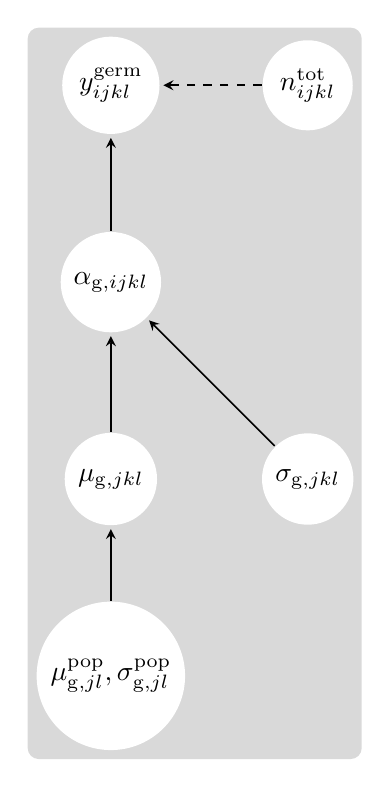
\begin{tikzpicture}[
            > = stealth, % arrow head style
            shorten > = 1pt, % don't touch arrow head to node
            auto,
            node distance = 2.5cm, % distance between nodes
            semithick % line style
        ]

        \tikzstyle{every state}=[
            draw = none,
            thick,
            fill = white,
            minimum size = 4mm
        ]


	% data level
        \node[state] (Y) [] {$y^{\mathrm{germ}}_{ijkl}$};
        \node[state] (N) [right of=Y] {$n^{\mathrm{tot}}_{ijkl}$};
       
        \path[dashed,->] (N) edge node {} (Y);

        % probability
        % \node[state] (T) [below of = Y] {$\theta_{ijk}$};
        %       
        % \path[->] (T) edge node {} (Y);
                  
                  % hyperparameters
         \node[state] (AB) [below of = Y] {$\alpha_{\mathrm{g},ijkl}$};
                
         \path[->] (AB) edge node {} (Y);
         
          % hyperparameters
        
         \node[state] (MS) [below of = AB] {$\mu_{\mathrm{g},jkl}$};
         \node[state] (A)[ right of = MS]  {$\sigma_{\mathrm{g},jkl}$};
         
         \path[->] (A) edge node {} (AB);       
         \path[->] (MS) edge node {} (AB);       
         
         \node[state] (H) [below of = MS] {$\mu^\mathrm{pop}_{\mathrm{g},jl},\sigma^\mathrm{pop}_{\mathrm{g},jl}$};
         \path[->] (H) edge node {} (MS);       
          
                    \begin{scope}[on background layer]
   \node [fit=(Y) (N) (H), fill= gray!30, rounded corners, inner sep=.1cm] {};
  \end{scope}
                 
  \end{tikzpicture}
  %
\subcaption{Directed acyclic graph for the hierarchical model for conditional germination. Solid arrows depict the relationships among random variables, and dashed arrows depict the deterministic relationships.}
\end{subfigure}
\end{figure}

\clearpage
\newpage

\subsubsection{Seed survival}
%%%%%%%%%%%%%%%%%%%%%%%%%%%%%%%%%%%%%%%%%%%%%%%%%%%%
% DIRECTED ACYCLIC GRAPHS FOR SEED DECAY MODEL
%%%%%%%%%%%%%%%%%%%%%%%%%%%%%%%%%%%%%%%%%%%%%%%%%%%%
\begin{figure}[h]%
\begin{subfigure}[c]{\textwidth}
\centering
   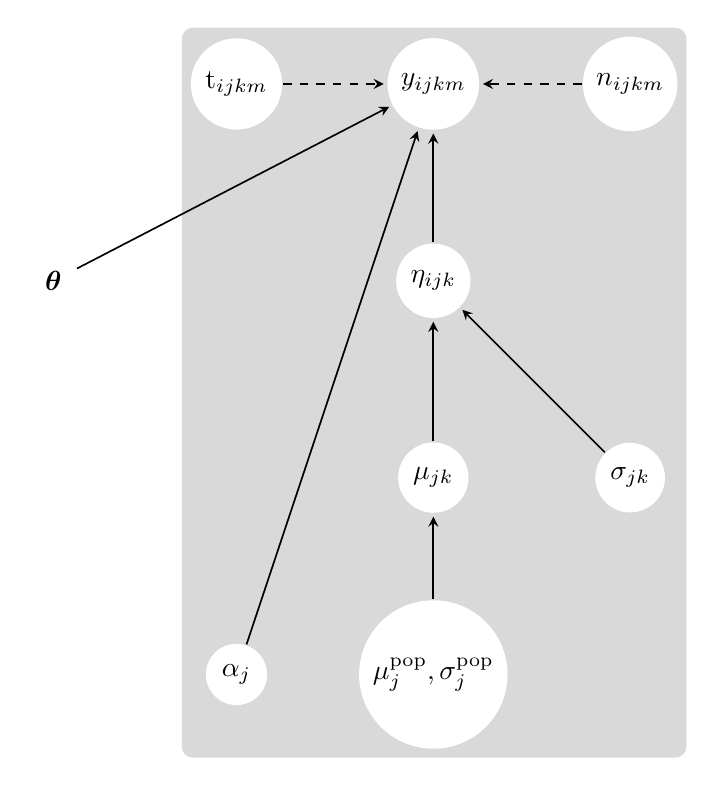
\begin{tikzpicture}[
            > = stealth, % arrow head style
            shorten > = 1pt, % don't touch arrow head to node
            auto,
            node distance = 2.5cm, % distance between nodes
            semithick % line style
        ]

        \tikzstyle{every state}=[
            draw = none,
            thick,
            fill = white,
            minimum size = 4mm
        ]


	% data level
        \node[state] (Y) [] {$y_{ijkm}$};
        \node[state] (N) [right of=Y] {$n_{ijkm}$};
        \node[state] (T) [left of = Y] {$\mathrm{t}_{ijkm}$};

        \path[dashed,->] (N) edge node {} (Y);

        % probability
        % \node[state] (T) [below of = Y] {$\gamma_{ijk}$};
        %       
        % \path[->] (T) edge node {} (Y);
        
       % \node[state] (LAT) [draw=none, thick, fill=white, minimum size=8mm,rounded rectangle, below of = Y] {$g(\eta_{ijk},\theta_{jkm})$};
        \path[dashed,->] (T) edge node {} (Y);

                  % hyperparameters
        \node[state] (AB) [below of = Y] {$\eta_{ijk}$};
       \node[state] (TH) [left = 4 cm of AB] {$\bm{\theta}$};
        
     %    \path[->] (LAT) edge node {} (Y);
         \path[->] (AB) edge node {} (Y);
         \path[->] (TH) edge node {} (Y);
         
          % hyperparameters
        
         \node[state] (MS) [below of = AB] {$\mu_{jk}$};
         \node[state] (A) [ right of = MS]  {$\sigma_{jk}$};
         
         \path[->] (A) edge node {} (AB);       
         \path[->] (MS) edge node {} (AB);       
         
         \node[state] (H) [below of = MS] {$\mu^\mathrm{pop}_{j},\sigma^\mathrm{pop}_{j}$};
         \path[->] (H) edge node {} (MS);       
         
         \node[state] (ALPHA) [left of = H] {$\alpha_{j}$};
         \path[->] (ALPHA) edge node {} (Y);       


          \begin{scope}[on background layer]
   \node [fit=(T) (N) (H), fill= gray!30, rounded corners, inner sep=.1cm] {};
  \end{scope}
  
  \end{tikzpicture}
  %
   \subcaption{Directed acyclic graphs for the models of seed survival. The parameter $\bm{\theta}$ links the conditional germination model to the seed survival model. Solid arrows depict the relationships among random variables, and dashed arrows depict the deterministic relationships.}
\end{subfigure}
\end{figure}

\clearpage
\newpage


\subsubsection{Seed survival from June to October}
%%%%%%%%%%%%%%%%%%%%%%%%%%%%%%%%%%%%%%%%%%%%%%%%%%%%
% DIRECTED ACYCLIC GRAPHS FOR SEED DECAY MODEL
%%%%%%%%%%%%%%%%%%%%%%%%%%%%%%%%%%%%%%%%%%%%%%%%%%%%
\begin{figure}[h]%
\begin{subfigure}[c]{\textwidth}
\centering
  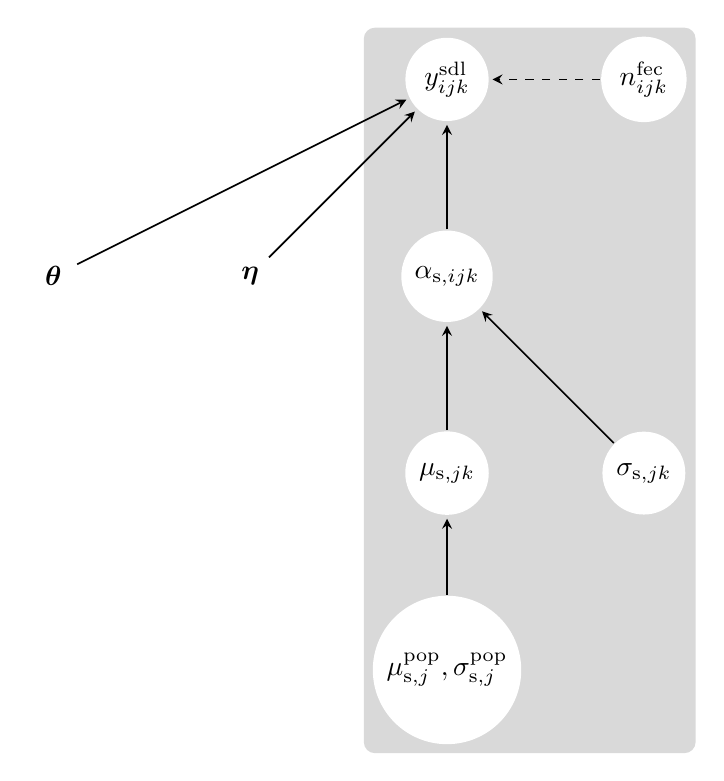
\begin{tikzpicture}[
            > = stealth, % arrow head style
            shorten > = 1pt, % don't touch arrow head to node
            auto,
            node distance = 2.5cm, % distance between nodes
            semithick % line style
        ]

        \tikzstyle{every state}=[
            draw = none,
            thick,
            fill = white,
            minimum size = 4mm
        ]


	% data level
        \node[state] (Y3) [] {$y^{\mathrm{sdl}}_{ijk}$};
        \node[state] (N3) [right of=Y3] {$n^{\mathrm{fec}}_{ijk}$};
       
        \path[dashed,->] (N3) edge node {} (Y3);

        % probability
        % \node[state] (T) [below of = Y] {$\theta_{ijk}$};
        %       
        % \path[->] (T) edge node {} (Y);
                  
                  % hyperparameters
         \node[state] (AB3) [below of = Y3] {$\alpha_{\mathrm{s},ijk}$};
        \node[state] (ETA3) [left of = AB3] {$\bm{\eta}$};
       \node[state] (TH3) [left of = ETA3] {$\bm{\theta}$};
               
         \path[->] (AB3) edge node {} (Y3);
         \path[->] (ETA3) edge node {} (Y3);
         \path[->] (TH3) edge node {} (Y3);
        
          % hyperparameters
        
         \node[state] (MS3) [below of = AB3] {$\mu_{\mathrm{s},jk}$};
         \node[state] (A3)[ right of = MS3]  {$\sigma_{\mathrm{s},jk}$};
         
         \path[->] (A3) edge node {} (AB3);       
         \path[->] (MS3) edge node {} (AB3);       
         
         \node[state] (H3) [below of = MS3] {$\mu^\mathrm{pop}_{\mathrm{s},j},\sigma^\mathrm{pop}_{\mathrm{s},j}$};
         \path[->] (H3) edge node {} (MS3);       
          
                    \begin{scope}[on background layer]
   \node [fit=(Y3) (N3) (H3), fill= gray!30, rounded corners, inner sep=.1cm] {};
  \end{scope}
                 
  \end{tikzpicture}        
 

  %
   \subcaption{Directed acyclic graphs for the models of seed survival from reproduction to October. The parameter $\bm{\theta}$ links the model to the conditional germination model. The parameter $\bm{\eta}$ links the model to the seed survival model. Solid arrows depict the relationships among random variables, and dashed arrows depict the deterministic relationships.}
\end{subfigure}
\end{figure}

\clearpage
\newpage



\subsubsection{Full model: germination, seed survivorship, initial seed survival}
%%%%%%%%%%%%%%%%%%%%%%%%%%%%%%%%%%%%%%%%%%%%%%%%%%%%
% DIRECTED ACYCLIC GRAPHS FOR SEED DECAY MODEL
%%%%%%%%%%%%%%%%%%%%%%%%%%%%%%%%%%%%%%%%%%%%%%%%%%%%
\begin{figure}[h]%
\begin{subfigure}[c]{\textwidth}
 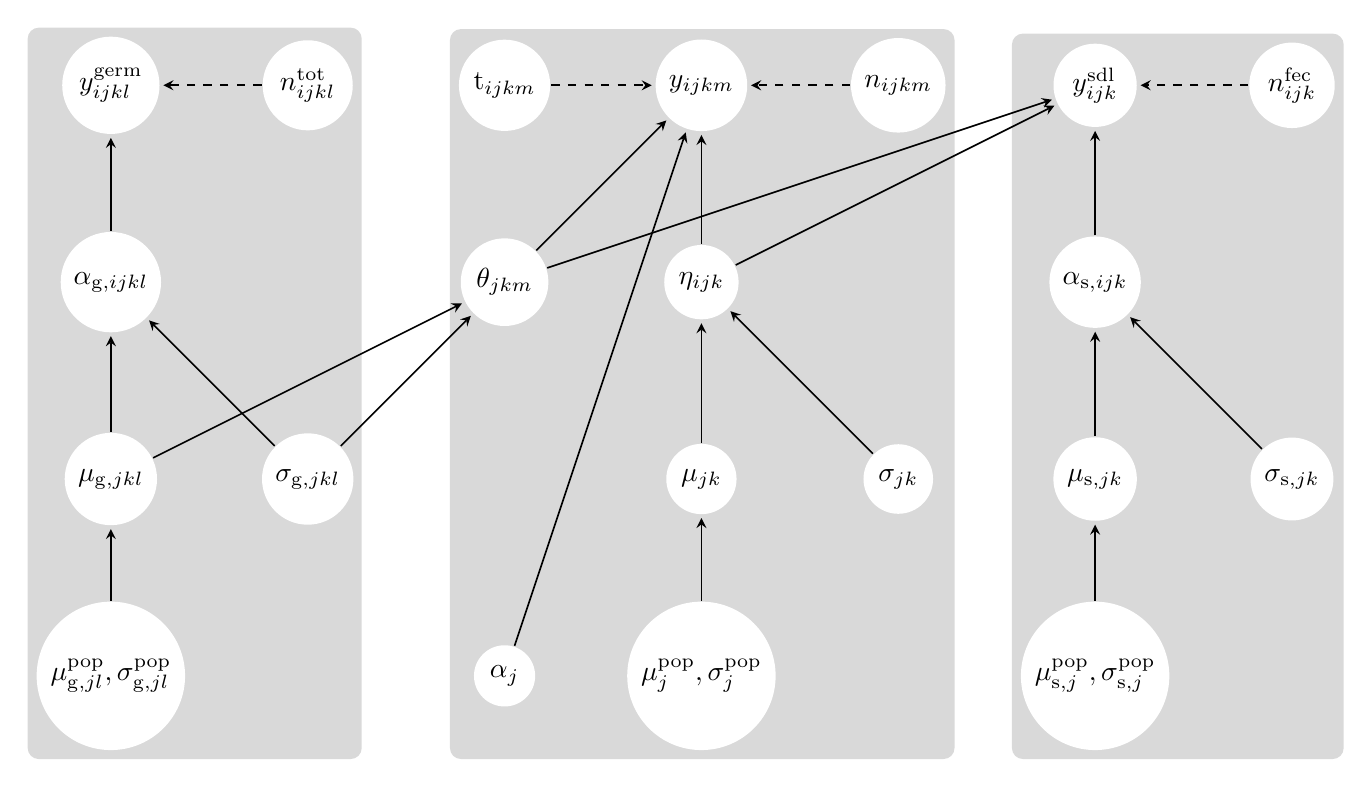
\begin{tikzpicture}[
            > = stealth, % arrow head style
            shorten > = 1pt, % don't touch arrow head to node
            auto,
            node distance = 2.5cm, % distance between nodes
            semithick % line style
        ]

        \tikzstyle{every state}=[
            draw = none,
            thick,
            fill = white,
            minimum size = 4mm
        ]


	% data level
        \node[state] (Y) [] {$y^{\mathrm{germ}}_{ijkl}$};
        \node[state] (N) [right of=Y] {$n^{\mathrm{tot}}_{ijkl}$};
       
        \path[dashed,->] (N) edge node {} (Y);
                  
         % hyperparameters
         \node[state] (AB) [below of = Y] {$\alpha_{\mathrm{g},ijkl}$};
                
         \path[->] (AB) edge node {} (Y);
         
          % hyperparameters
        
         \node[state] (MS) [below of = AB] {$\mu_{\mathrm{g},jkl}$};
         \node[state] (A)[ right of = MS]  {$\sigma_{\mathrm{g},jkl}$};
         
         \path[->] (A) edge node {} (AB);       
         \path[->] (MS) edge node {} (AB);       
         
         \node[state] (H) [below of = MS] {$\mu^\mathrm{pop}_{\mathrm{g},jl},\sigma^\mathrm{pop}_{\mathrm{g},jl}$};
         \path[->] (H) edge node {} (MS);       
          
         %% SURVIVAL

	% data level
        \node[state] (T2) [right of = N] {$\mathrm{t}_{ijkm}$};
        \node[state] (Y2) [right of = T2] {$y_{ijkm}$};
        \node[state] (N2) [right of=Y2] {$n_{ijkm}$};

        \path[dashed,->] (N2) edge node {} (Y2);

        \path[dashed,->] (T2) edge node {} (Y2);

                  % hyperparameters
        \node[state] (AB2) [below of = Y2] {$\eta_{ijk}$};
       \node[state] (TH2) [left of = AB2] {$\theta_{jkm}$};
        
         \path[->] (AB2) edge node {} (Y2);
         \path[->] (TH2) edge node {} (Y2);
         \path[->] (MS) edge node {} (TH2);
          \path[->] (A) edge node {} (TH2);
                  
          % hyperparameters
        
         \node[state] (MS2) [below of = AB2] {$\mu_{jk}$};
         \node[state] (A2) [ right of = MS2]  {$\sigma_{jk}$};
         
         \path[->] (A2) edge node {} (AB2);       
         \path[->] (MS2) edge node {} (AB2);       
         
         \node[state] (H2) [below of = MS2] {$\mu^\mathrm{pop}_{j},\sigma^\mathrm{pop}_{j}$};
         \path[->] (H2) edge node {} (MS2);       
         
         \node[state] (ALPHA2) [left of = H2] {$\alpha_{j}$};
         \path[->] (ALPHA2) edge node {} (Y2);       

         % INITIAL SURVIVAL

	% data level
        \node[state] (Y3) [right of =N2] {$y^{\mathrm{sdl}}_{ijk}$};
        \node[state] (N3) [right of=Y3] {$n^{\mathrm{fec}}_{ijk}$};
       
        \path[dashed,->] (N3) edge node {} (Y3);
                   
        % hyperparameters
         \node[state] (AB3) [below of = Y3] {$\alpha_{\mathrm{s},ijk}$};
               
         \path[->] (AB3) edge node {} (Y3);
         \path[->] (AB2) edge node {} (Y3);
         \path[->] (TH2) edge node {} (Y3);
        
          % hyperparameters
        
         \node[state] (MS3) [below of = AB3] {$\mu_{\mathrm{s},jk}$};
         \node[state] (A3)[ right of = MS3]  {$\sigma_{\mathrm{s},jk}$};
         
         \path[->] (A3) edge node {} (AB3);       
         \path[->] (MS3) edge node {} (AB3);       
         
         \node[state] (H3) [below of = MS3] {$\mu^\mathrm{pop}_{\mathrm{s},j},\sigma^\mathrm{pop}_{\mathrm{s},j}$};
         \path[->] (H3) edge node {} (MS3);       
         
         
         % BACKGROUND


          \begin{scope}[on background layer]
   \node [fit=(T2) (N2) (H2), fill= gray!30, rounded corners, inner sep=.1cm] {};
   \node [fit=(Y) (N) (H), fill= gray!30, rounded corners, inner sep=.1cm] {};
   \node [fit=(Y3) (N3) (H3), fill= gray!30, rounded corners, inner sep=.1cm] {};
  \end{scope}
  
  \end{tikzpicture}
  %
   \subcaption{Directed acyclic graphs for the full model. Models for each set of data are encapsulated in a gray box; links among the datasets are shown by arrows that cross over between boxes. Solid arrows depict the relationships among random variables, and dashed arrows depict the deterministic relationships.}
\end{subfigure}
\end{figure}



\clearpage
\newpage



\section{Viability trials}\label{section-3}

\subsection{Data}

We collected the following data during the viability trials: 

\begin{itemize}
	\item $n^{\mathrm{germ}}_{ijkl}$ = observed count of seeds at the start of the germination trial for the $i^{th}$ bag, from the $j^{th}$ population, in the $k^{th}$ experimental year, for seeds of age $l$, assumed to be measured perfectly
	\item $y^{\mathrm{germ}}_{ijk}$ = observed count of germinated seedlings in the germination trial for the $i^{th}$ bag, from the $j^{th}$ population, in the $k^{th}$ year, for seeds of age $l$, assumed to be measured perfectly 
	\item $n^{\mathrm{viab}}_{ijk}$ = observed count of seeds at the start of the viability trial for the $i^{th}$ bag, from the $j^{th}$ population, in the $k^{th}$ year, for seeds of age $l$, assumed to be measured perfectly 
	\item $y^{\mathrm{viab}}_{ijk}$ = observed count of viable seedlings in the viability trial for the $i^{th}$ bag, from the $j^{th}$ population, in the $k^{th}$ year, for seeds of age $l$, assumed to be measured perfectly 
\end{itemize}

\subsection{Model}

All data from viability trials is in the form of binomial trials: we have counts of seeds at the start and end of an experimental window of time. All models have the same structure for seeds in bag $i$ in population $j$ in experimental year $k$. If the number of seeds starting the trial (trials) is $n_{ijk}$ and the number of seeds at the end of the trial (successes) is $y_{ijk}$, we write a model that has a population-level mean and year-level means drawn from the population-level distribution. Broadly, this is two-level hierarchical model with a population-level mean, and year-level means drawn from the population-level distribution. The probability of success for each bag is drawn from this year- and population-level distribution. The model uses a binomial likelihood. The joint posterior for viability trials thus has the following general form:
%
\begin{align}
  \begin{split}
 [  \bm{\alpha_G} , \bm{\mu_G} , \bm{\sigma_G} , \bm{\mu^\mathrm{pop}_G}, \bm{\sigma^\mathrm{pop}_G} | & \bm{y^{\mathrm{tot}}}  ] \propto \prod_{i=1}^{I}   \prod_{j=1}^{J}  \prod_{k=1}^{K} 
   \mathrm{binomial} ( y^{\mathrm{germ}}_{ijk} | n^\mathrm{test_g}_{ijk}, \mathrm{logit}^{-1}( \alpha_{G,ijk} ) ) 
   \\ & \times \mathrm{normal} ( \alpha_{G,ijk}  | \mu_{G,jk}, \sigma{_{G,jk} })
  \\ & \times \mathrm{normal} ( \mu_{G,jk}  | \mu^\mathrm{pop}_{G,j}, \sigma^\mathrm{pop}_{G,j} )
  \\ & \times \textrm{half-normal} ( \sigma_{G,jk} | 0,1)
  \\ & \times \mathrm{normal} ( \mu^\mathrm{pop}_{G,j} | 0 , 1000 ) \textrm{half-normal} ( \sigma^\mathrm{pop}_{G,j} | 0,1).
  \end{split}
\end{align}
%
\begin{align}
  \begin{split}
 [  \bm{\alpha_V} , \bm{\mu_V} , \bm{\sigma_V} , \bm{\mu^\mathrm{pop}_V}, \bm{\sigma^\mathrm{pop}_V} | & \bm{y^{\mathrm{tot}}}  ] \propto \prod_{i=1}^{I}   \prod_{j=1}^{J}  \prod_{k=1}^{K} 
   \mathrm{binomial} ( y^{\mathrm{viab}}_{ijk} | n^\mathrm{test_v}_{ijk}, \mathrm{logit}^{-1}( \alpha_{V,ijk} ) ) 
   \\ & \times \mathrm{normal} ( \alpha_{V,ijk}  | \mu_{V,jk}, \sigma{_{V,jk} })
  \\ & \times \mathrm{normal} ( \mu_{V,jk}  | \mu^\mathrm{pop}_{V,j}, \sigma^\mathrm{pop}_{V,j} )
  \\ & \times \textrm{half-normal} ( \sigma_{V,jk} | 0,1)
  \\ & \times \mathrm{normal} ( \mu^\mathrm{pop}_{V,j} | 0 , 1000 ) \textrm{half-normal} ( \sigma^\mathrm{pop}_{V,j} | 0,1).
  \end{split}
\end{align}

\newpage
\clearpage

\subsection{Directed acyclic graphs}

%%%%%%%%%%%%%%%%%%%%%%%%%%%%%%%%%%%%%%%%%%%%%%%%%%%%
% DIRECTED ACYCLIC GRAPHS FOR VIABILITY TRIALS
%%%%%%%%%%%%%%%%%%%%%%%%%%%%%%%%%%%%%%%%%%%%%%%%%%%%
\begin{figure}[h]%
\begin{subfigure}[c]{\textwidth}
\centering
   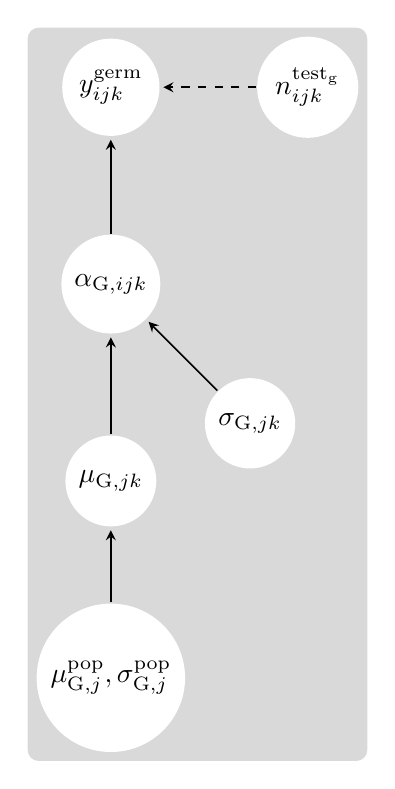
\begin{tikzpicture}[
            > = stealth, % arrow head style
            shorten > = 1pt, % don't touch arrow head to node
            auto,
            node distance = 2.5cm, % distance between nodes
            semithick % line style
        ]

        \tikzstyle{every state}=[
            draw = none,
            thick,
            fill = white,
            minimum size = 4mm
        ]F


	% data level
        \node[state] (Y) [] {$y^{\mathrm{germ}}_{ijk}$};
        \node[state] (N) [right of=Y] {$n^\mathrm{test_g}_{ijk}$};
       
        \path[dashed,->] (N) edge node {} (Y);

        % probability
        % \node[state] (T) [below of = Y] {$\theta_{ijk}$};
        %       
        % \path[->] (T) edge node {} (Y);
                  
                  % hyperparameters
         \node[state] (AB) [below of = Y] {$\alpha_{\mathrm{G},ijk}$};
                
         \path[->] (AB) edge node {} (Y);
         
          % hyperparameters
        
         \node[state] (MS) [below of = AB] {$\mu_{\mathrm{G},jk}$};
         \node[state] (A) [below right of = AB] {$\sigma_{\mathrm{G},jk}$};
         
         \path[->] (A) edge node {} (AB);       
         \path[->] (MS) edge node {} (AB);       
         
         \node[state] (H) [below of = MS] {$\mu^\mathrm{pop}_{\mathrm{G},j},\sigma^\mathrm{pop}_{\mathrm{G},j}$};
         \path[->] (H) edge node {} (MS);       

                    \begin{scope}[on background layer]
   \node [fit=(Y) (N) (H), fill= gray!30, rounded corners, inner sep=.1cm] {};
  \end{scope}
  
  \end{tikzpicture}
  %
    \hspace{1cm}% NO SPACE!
  % BEGIN FIGURE 3
   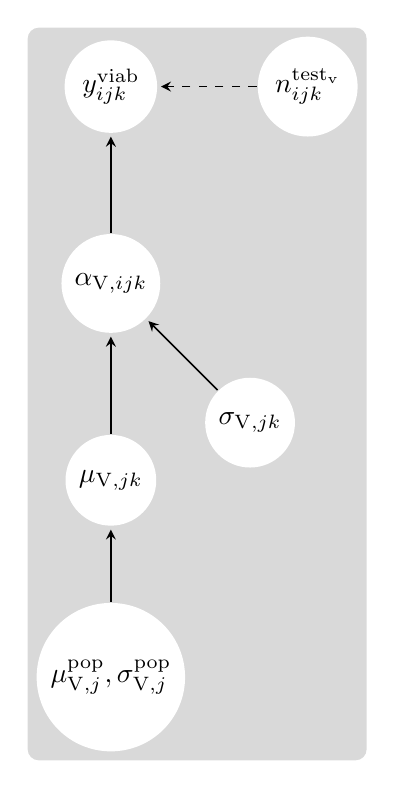
\begin{tikzpicture}[
            > = stealth, % arrow head style
            shorten > = 1pt, % don't touch arrow head to node
            auto,
            node distance = 2.5cm, % distance between nodes
            semithick % line style
        ]

        \tikzstyle{every state}=[
            draw = none,
            thick,
            fill = white,
            minimum size = 4mm
        ]F


	% data level
        \node[state] (Y) [] {$y^{\mathrm{viab}}_{ijk}$};
        \node[state] (N) [right of=Y] {$n^\mathrm{test_v}_{ijk}$};
       
        \path[dashed,->] (N) edge node {} (Y);

        % probability
        % \node[state] (T) [below of = Y] {$\theta_{ijk}$};
        %       
        % \path[->] (T) edge node {} (Y);
                  
                  % hyperparameters
         \node[state] (AB) [below of = Y] {$\alpha_{\mathrm{V},ijk}$};
                
         \path[->] (AB) edge node {} (Y);
         
          % hyperparameters
        
         \node[state] (MS) [below of = AB] {$\mu_{\mathrm{V},jk}$};
         \node[state] (A) [below right of = AB] {$\sigma_{\mathrm{V},jk}$};
         
         \path[->] (A) edge node {} (AB);       
         \path[->] (MS) edge node {} (AB);       
         
         \node[state] (H) [below of = MS] {$\mu^\mathrm{pop}_{\mathrm{V},j},\sigma^\mathrm{pop}_{\mathrm{V},j}$};
         \path[->] (H) edge node {} (MS);      
         
                             \begin{scope}[on background layer]
   \node [fit=(Y) (N) (H), fill= gray!30, rounded corners, inner sep=.1cm] {};
  \end{scope}
                                
  \end{tikzpicture}
\subcaption{Directed acyclic graphs for the hierarchical models for viability trials. Solid arrows depict the relationships among random variables, and dashed arrows depict the deterministic relationships.}
\end{subfigure}
\end{figure}

\section{Estimated parameters to model parameters}\label{section-4}

We now use the parameter estimates from Section \ref{section-2} and \ref{section-3} to obtain the parameters for the structured population model from Section \ref{section-1}. Below, we describe how we obtained population-level estimates for the parameters in Table \ref{tab:structured-parameters}.

First, we use the full model for germination, seed survival, and initial seed survival to obtain population-level estimates for the survival functions for seed persistence and age-specific germination. We use the posterior distributions for the population-level mean of the inverse-scale parameter ($\mu_j^\mathrm{pop}$) and the shape parameter ($\alpha_j$) to derive (\hl{semantics: marginalize to obtain?}) the population-level parameters for the Weibull survival function. We transform the population-level posterior distributions for the survival probability from the latent scale to $[0,1]$ by taking the inverse logit; this transforms the parameters into the probability of success.

We then use the posterior distributions for the population-level mean of the probability of germination on the latent scale ($\mu^\mathrm{pop}_{\mathrm{g},jl}$) to derive the age-specific germination probabilities. We transform the population-level posterior distributions for the germination probability from the latent scale to $[0,1]$ by taking the inverse logit; this transforms the parameters into the probability of success.

We use the product of the Weibull survival function and the germination histories (as in Section \ref{section-2}) to obtain the survival functions associated with persistence of seeds in the soil seed bank ($\theta_\cdot$ in Table \ref{tab:survival-functions}). At this point, we switch from continuous time to the discrete times in Table \ref{tab:survival-functions}) by calculating the survival at those times. 

We then estimate viability with the posterior distributions for the population-level mean of the probability of germination and viability from the viability trials. For estimates of viability in October, we transform the values from the latent scale ($\mu^\mathrm{pop}_{\mathrm{G},j}$, $\mu^\mathrm{pop}_{\mathrm{V},j}$) to the probability scale ($\theta_G$, $\theta_V$. We estimate the overall probability of viability, $\nu$, as $\theta_g + \theta_v (1-\theta_g)$. This weights the estimates relative to the probability of germination (eg. if no seeds germinate the estimate of viability will mostly come from the viability test). For estimates of viability in January, we interpolate between estimates of viability on the latent scale before transforming interpolated values to the probability scale. This allows us to retain the uncertainty associated with our estimates of viability. We transform the population-level posterior distributions for the overall probability of viability from the latent scale to $[0,1]$ by taking the inverse logit; this transforms the parameters into the probability of success.

With all of these pieces in hand, we calculate values of $\phi$, which are the probability of seed persistence and viability. We then estimate the probability of germination conditional on viability as in Table \ref{tab:structured-parameters}.

\newpage

\section*{Figures}

 \begin{figure}[!h]
   \centering
       \includegraphics[page=1,width=1\textwidth]{../../manuscript/figures/seed-bag-figure.pdf}  
    \caption{ Summary of the seed bag burial experiments and viability trials. \hl{Figure will be labeled as (A: seed bag trials , B: viability trials, C: germination probability, D: survival probability. }. (A) The gray panel contains a graphical representation of the seed bag trials. Seeds were buried at the start of each experiment (100 seeds in month 0). Seed bags were unearthed and intact seeds ($y_{\cdot \cdot}$) and germinants ($y_{\mathrm{g},\cdot}$ counted. The graph below the panel shows a hypothetical survival function associated with persistence of seeds in the soil seed bank. (B) The gray panel contains a graphical representation of the viability trials. Seeds were tested in two rounds; germination trials were performed and then some or all of the ungerminated seeds were tested for viability. The graph below the panel shows hypothetical data from a series of viability trials and the interpolated, inferred viabilities at times when viability was unobserved. (C) Age-specific germination probably is summarized in three ways. (D) The graph shows the survival function for persistence of seeds in the soil seed bank (black line) and the estimated discrete survival probabilities for persistence and viability of seeds (orange points). }
 \label{fig:seed-bag-experiments}
\end{figure}



%%%%%%%%%%%%%%%%%%%%%%%%%%%%%%%%%%%%%%%%%%%%%%%%%%%%
% DIRECTED ACYCLIC GRAPHS FOR AGE 1 SEED BAGS
%%%%%%%%%%%%%%%%%%%%%%%%%%%%%%%%%%%%%%%%%%%%%%%%%%%%
\begin{figure}[h]%
\begin{subfigure}[c]{\textwidth}
   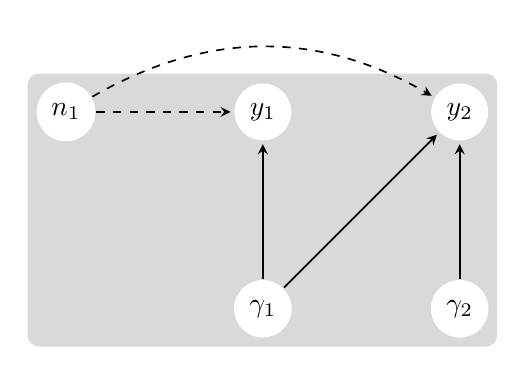
\begin{tikzpicture}[
            > = stealth, % arrow head style
            shorten > = 1pt, % don't touch arrow head to node
            auto,
            node distance = 2.5cm, % distance between nodes
            semithick % line style
        ]

        \tikzstyle{every state}=[
            draw = none,
            thick,
            fill = white,
            minimum size = 4mm
        ]


	% data level
        \node[state] (Y) [] {$y_1$};
        \node[state] (N) [left of=Y] {$n_1$};
        \node[state] (Y2) [right of=Y] {$y_2$};
       
        \path[dashed,->] (N) edge node {} (Y);
        \path[dashed,->,bend left] (N) edge node {} (Y2);

         % parameters
         \node[state] (AB) [below of = Y] {$\gamma_1$};
         \node[state] (AB2) [below of = Y2] {$\gamma_2$};
                
         \path[->] (AB) edge node {} (Y);
         \path[->] (AB) edge node {} (Y2);
         \path[->] (AB2) edge node {} (Y2);
         
          \begin{scope}[on background layer]
   	  \node [fit=(N) (Y2) (AB), fill= gray!30, rounded corners, inner sep=.1cm] {};
          \end{scope}
          
  \end{tikzpicture}
  %
    \hspace{1cm}% NO SPACE!
  % BEGIN FIGURE 3
   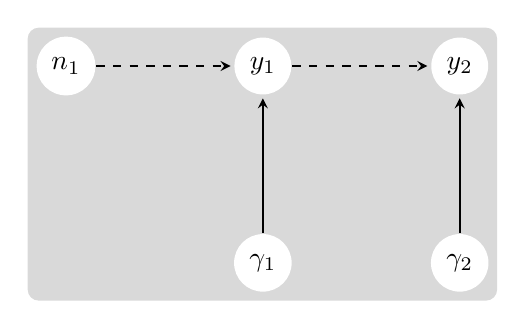
\begin{tikzpicture}[
              > = stealth, % arrow head style
            shorten > = 1pt, % don't touch arrow head to node
            auto,
            node distance = 2.5cm, % distance between nodes
            semithick % line style
        ]

        \tikzstyle{every state}=[
            draw = none,
            thick,
            fill = white,
            minimum size = 4mm
        ]


	% data level
        \node[state] (Y) [] {$y_1$};
        \node[state] (N) [left of=Y] {$n_1$};
         \node[state] (Y2) [right of=Y] {$y_2$};
       
        \path[dashed,->] (N) edge node {} (Y);
        \path[dashed,->] (Y) edge node {} (Y2);

         % parameters
         \node[state] (AB) [below of = Y] {$\gamma_1$};
         \node[state] (AB2) [below of = Y2] {$\gamma_2$};
                
         \path[->] (AB) edge node {} (Y);
         \path[->] (AB2) edge node {} (Y2);
         
          \begin{scope}[on background layer]
   	  \node [fit=(N) (Y2) (AB), fill= gray!30, rounded corners, inner sep=.1cm] {};
          \end{scope}
                           
  \end{tikzpicture}
  %
\subcaption{Directed acyclic graphs for the hierarchical models for seed bag rates. Solid arrows depict the relationships among random variables, and dashed arrows depict the deterministic relationships.}
\end{subfigure}
\end{figure}


%%%%%%%%%%%%%%%%%%%%%%%%%%%%%%%%%%%%%%%%%%%%%%%%%%%%
% POSTERIOR AND JOINT DISTRIBUTIONS FOR AGE 1 SEED BAGS
%%%%%%%%%%%%%%%%%%%%%%%%%%%%%%%%%%%%%%%%%%%%%%%%%%%%

% QUESTIONS
% do I need to include \bm{n} on the RHS of the conditional statement for the posterior?

\begin{align}
  \begin{split}
 [  \gamma_1, \gamma_2  | & \bm{y_1} , \bm{y_2} ] \propto 
   \mathrm{binomial} ( y_1 | n_1, \mathrm{logit}^{-1}( \alpha_1 ) )  
      \\ & \times \mathrm{binomial} ( y_2 | n_1, \mathrm{logit}^{-1}( \alpha_1 ) \times \mathrm{logit}^{-1}( \alpha_2 ) ) 
   \\ & \times \mathrm{normal} ( \alpha_1  | \mu_1, \sigma_1 ) \mathrm{normal} ( \alpha_2  | \mu_2, \sigma_2 )
  \\ & \times \mathrm{normal} ( \mu_1 | 0 , 1000 ) \textrm{half-normal} ( \sigma_1 | 0,1)
    \\ & \times \mathrm{normal} ( \mu_2 | 0 , 1000 ) \textrm{half-normal} ( \sigma_2 | 0,1).
  \end{split}
\end{align}
%
\begin{align}
  \begin{split}
 [  \gamma_1, \gamma_2  | & \bm{y_1} , \bm{y_2} ] \propto 
   \mathrm{binomial} ( y_1 | n_1, \mathrm{logit}^{-1}( \alpha_1 ) )
      \\ & \times  \mathrm{binomial} ( y_2 | y_1, \mathrm{logit}^{-1}( \alpha_2 ) ) 
   \\ & \times \mathrm{normal} ( \alpha_1  | \mu_1, \sigma_1 ) \mathrm{normal} ( \alpha_2  | \mu_2, \sigma_2 )
  \\ & \times \mathrm{normal} ( \mu_1 | 0 , 1000 ) \textrm{half-normal} ( \sigma_1 | 0,1)
    \\ & \times \mathrm{normal} ( \mu_2 | 0 , 1000 ) \textrm{half-normal} ( \sigma_2 | 0,1).
  \end{split}
\end{align}
%

\clearpage
\newpage



\subsection*{Identifiability across years}
%%%%%%%%%%%%%%%%%%%%%%%%%%%%%%%%%%%%%%%%%%%%%%%%%%%%
% DIRECTED ACYCLIC GRAPHS FOR AGE 1 SEED BAGS
%%%%%%%%%%%%%%%%%%%%%%%%%%%%%%%%%%%%%%%%%%%%%%%%%%%%
\begin{figure}[h]%
\begin{subfigure}[c]{\textwidth}
   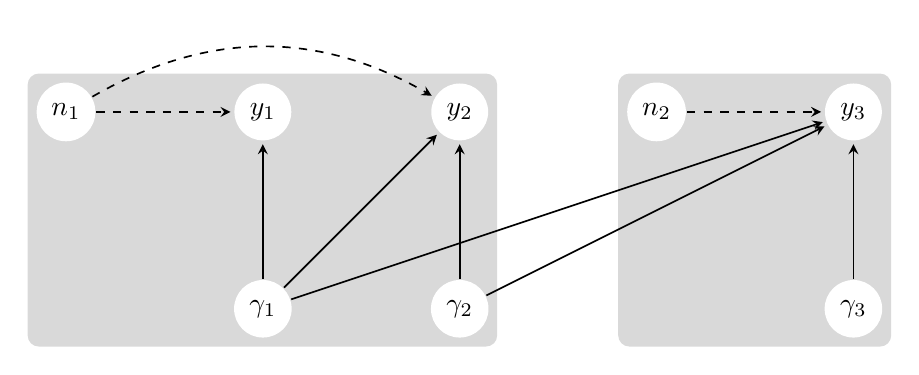
\begin{tikzpicture}[
            > = stealth, % arrow head style
            shorten > = 1pt, % don't touch arrow head to node
            auto,
            node distance = 2.5cm, % distance between nodes
            semithick % line style
        ]

        \tikzstyle{every state}=[
            draw = none,
            thick,
            fill = white,
            minimum size = 4mm
        ]


	% data level
        \node[state] (Y) [] {$y_1$};
        \node[state] (N) [left of=Y] {$n_1$};
        \node[state] (Y2) [right of=Y] {$y_2$};
        \node[state] (N2) [right of=Y2] {$n_2$};
        \node[state] (Y3) [right of=N2] {$y_3$};
       
        \path[dashed,->] (N) edge node {} (Y);
        \path[dashed,->,bend left] (N) edge node {} (Y2);
        \path[dashed,->] (N2) edge node {} (Y3);

         % parameters
         \node[state] (AB) [below of = Y] {$\gamma_1$};
         \node[state] (AB2) [below of = Y2] {$\gamma_2$};
         \node[state] (AB3) [below of = Y3] {$\gamma_3$};
                
         \path[->] (AB) edge node {} (Y);
         \path[->] (AB) edge node {} (Y2);
         \path[->] (AB2) edge node {} (Y2);
         \path[->] (AB) edge node {} (Y3);
         \path[->] (AB2) edge node {} (Y3);
         \path[->] (AB3) edge node {} (Y3);
         
          \begin{scope}[on background layer]
   	  \node [fit=(N) (Y2) (AB),fill=gray!30, rounded corners, inner sep=.1cm] {};
	  \node [fit=(N2) (Y3) (AB3),fill=gray!30, rounded corners, inner sep=.1cm] {};
          \end{scope}
          
  \end{tikzpicture} \\ \\ \\
   % BEGIN FIGURE 3
 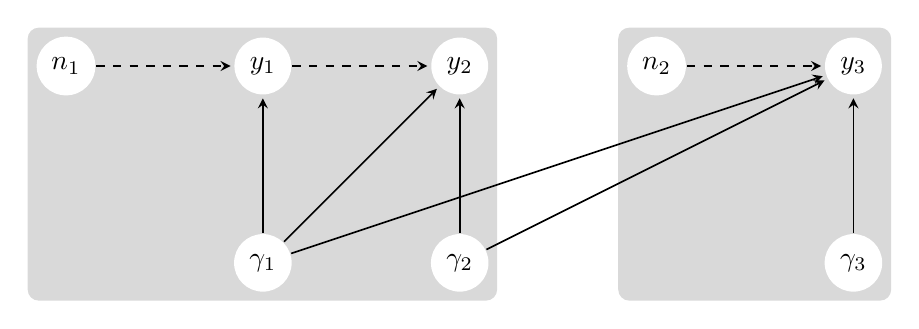
\begin{tikzpicture}[
            > = stealth, % arrow head style
            shorten > = 1pt, % don't touch arrow head to node
            auto,
            node distance = 2.5cm, % distance between nodes
            semithick % line style
        ]

        \tikzstyle{every state}=[
            draw = none,
            thick,
            fill = white,
            minimum size = 4mm
        ]


	% data level
        \node[state] (Y) [] {$y_1$};
        \node[state] (N) [left of=Y] {$n_1$};
        \node[state] (Y2) [right of=Y] {$y_2$};
        \node[state] (N2) [right of=Y2] {$n_2$};
        \node[state] (Y3) [right of=N2] {$y_3$};
       
        \path[dashed,->] (N) edge node {} (Y);
        \path[dashed,->] (Y) edge node {} (Y2);
        \path[dashed,->] (N2) edge node {} (Y3);

         % parameters
         \node[state] (AB) [below of = Y] {$\gamma_1$};
         \node[state] (AB2) [below of = Y2] {$\gamma_2$};
         \node[state] (AB3) [below of = Y3] {$\gamma_3$};
                
         \path[->] (AB) edge node {} (Y);
         \path[->] (AB) edge node {} (Y2);
         \path[->] (AB2) edge node {} (Y2);
         \path[->] (AB) edge node {} (Y3);
         \path[->] (AB2) edge node {} (Y3);
         \path[->] (AB3) edge node {} (Y3);
         
          \begin{scope}[on background layer]
   	  \node [fit=(N) (Y2) (AB),fill=gray!30, rounded corners, inner sep=.1cm] {};
	  \node [fit=(N2) (Y3) (AB3),fill=gray!30, rounded corners, inner sep=.1cm] {};
          \end{scope}
          
  \end{tikzpicture}
  %
\subcaption{Directed acyclic graphs for the hierarchical models for seed bag rates. Solid arrows depict the relationships among random variables, and dashed arrows depict the deterministic relationships.}
\end{subfigure}
\end{figure}
%
%%%%%%%%%%%%%%%%%%%%%%%%%%%%%%%%%%%%%%%%%%%%%%%%%%%%
% POSTERIOR AND JOINT DISTRIBUTIONS FOR AGE 1 SEED BAGS
%%%%%%%%%%%%%%%%%%%%%%%%%%%%%%%%%%%%%%%%%%%%%%%%%%%%

% QUESTIONS
% do I need to include \bm{n} on the RHS of the conditional statement for the posterior?

\begin{align}
  \begin{split}
 [  \gamma_1, \gamma_2  | & \bm{y_1} , \bm{y_2} ] \propto 
   \mathrm{binomial} ( y_1 | n_1, \mathrm{logit}^{-1}( \alpha_1 ) )  
      \\ & \times \mathrm{binomial} ( y_2 | n_1, \mathrm{logit}^{-1}( \alpha_1 ) \times \mathrm{logit}^{-1}( \alpha_2 ) ) 
   \\ & \times \mathrm{normal} ( \alpha_1  | \mu_1, \sigma_1 ) \mathrm{normal} ( \alpha_2  | \mu_2, \sigma_2 )
  \\ & \times \mathrm{normal} ( \mu_1 | 0 , 1000 ) \textrm{half-normal} ( \sigma_1 | 0,1)
    \\ & \times \mathrm{normal} ( \mu_2 | 0 , 1000 ) \textrm{half-normal} ( \sigma_2 | 0,1).
  \end{split}
\end{align}
%
\begin{align}
  \begin{split}
 [  \gamma_1, \gamma_2  | & \bm{y_1} , \bm{y_2} ] \propto 
   \mathrm{binomial} ( y_1 | n_1, \mathrm{logit}^{-1}( \alpha_1 ) )
      \\ & \times  \mathrm{binomial} ( y_2 | y_1, \mathrm{logit}^{-1}( \alpha_2 ) ) 
   \\ & \times \mathrm{normal} ( \alpha_1  | \mu_1, \sigma_1 ) \mathrm{normal} ( \alpha_2  | \mu_2, \sigma_2 )
  \\ & \times \mathrm{normal} ( \mu_1 | 0 , 1000 ) \textrm{half-normal} ( \sigma_1 | 0,1)
    \\ & \times \mathrm{normal} ( \mu_2 | 0 , 1000 ) \textrm{half-normal} ( \sigma_2 | 0,1).
  \end{split}
\end{align}
%

\clearpage
\newpage



%% NEXT: DESCRIBE THE SURVIVAL FUNCTION FOR WEIBULL RESIDENCE TIME


In constructing our survival function, we have two types of data for each experimental year and age. Counts from January represent totals from prior to the germination of seeds of that age. The survival function of seeds at time $T$, $S^1_{ya}(T)$, for these counts in each experimental year $y$ is described by 
%
%\begin{align}
%  \begin{split}
%S^1_{ya} = P(T>a | Y=y) = 1 - \sum_{j=1}^{a} \gamma_{ya}
%  \end{split}
%\end{align}
%

% SOMETHING WRONG WITH THIS
\begin{align}
  \begin{split}
S^\mathrm{jan}_{a} = \prod_{j=1}^{a} (1- \gamma_{yj} )^{I(j=j-1)}
  \end{split}
\end{align}

Counts from October represent totals from after  the germination of seeds of that age. The survival function of seeds at time $T$, $S^2_{ya}(T)$, for these counts in each experimental year $y$ is described by
%
\begin{align}
  \begin{split}
S^\mathrm{oct}_{a} = \prod_{j=1}^{a} (1- \gamma_{yj} )
  \end{split}
\end{align}
%

The functions $S^\mathrm{jan}$ and $S^\mathrm{oct}$ describe the probability that a seed with a particular event (germination) history survives to January and October, respectively. 

To include both types of data in the seed bag experiment model, I combined the two functions and introduced an additional index for the type of data the function describes. The index $d=1,2$ now represents whether the data are counts from January ($d=1$) or October ($d=2$)
%
\begin{align}
  \begin{split}
S_{da} =  \prod_{j=1}^{a} \prod_{i=1}^{d}  (1- \gamma_{yj} )^{I(d=2)}
  \end{split}
\end{align}
%

%


The probability described below could probably be expressed compactly with indicator functions but I'm running into blocks on getting this to work. Below, $I(\cdot)$ is an indicator function that takes on the value of 1 when the statement in parentheses is true and the value of 0 when the statement in parentheses is false.

The first indicator function indicates whether we are observing the total number of seedlings in January (before germination).


\clearpage
$ \gamma_{jkl} = (1-\gamma_{1_{kl}})^{(1-I(j=1 \land l=1))} \times (1-\gamma_{2_{kl}})^{(1-I(j=1 \land l=2))} \times (1-\gamma_{3_{kl}})^{(1-I(j=1 \land l=3))}$


\clearpage

The models below represent the joint likelihood for data from the seed bag experiments. All data from seed bags and viability trials is in the form of binomial trials: we have counts of seeds at the start and end of an experimental window of time. All models for the parameters $\gamma_1, \gamma_2, \gamma_3, \gamma_4, \gamma_5$ have the same structure for seeds in bag $i$ in year $j$ in population $k$. If the number of seeds starting the trial (trials) is $n_{ijk}$ and the number of seeds at the end of the trial (successes) is $y_{ijk}$, we write a model that has a population-level mean and year-level means drawn from the population-level distribution. The probability of success for each bag is drawn from this year- and population-level distribution:

I compared convergence diagnostics (R-hat, effective sample size) for centered and non-centered parameterizations of the model. Here, I use the centered parameterization because this led to improved convergence. In each model, we obtain the population-level posterior distribution probability of success (the $\gamma$s) by marginalizing across years and taking the inverse logit.

The seed bank experiments might used to obtain age-specific survival and recruitment terms. So the terms could be survival to month 3 (equal to age-specific survival at midpoint), germination at month 3, survival from month 3 to month 12 (equal to age-specific survival at midpoint), germination at month 15, survival from month 15 to 24, germination at month 27, survival from month 27 to 36. There are some errors in the data still, need to look at those. For germination there is no clear pattern to germination, either for individual sites or across sites. There are monotonic increases, monotonic decreases, and nonmonotonic patterns. Might also help to look at viability across age. 

The seed pot experiments seem like they would be amenable to the kind of functions fit in the paper by Rees and Long. In those cases there are only 3 time points which would limit the application of the empirical seedling recruitment curves. But perhaps overlaying them per population would allow us to figure out whether there is consistency across years or whether particular cohorts follow different curves, and how this varies in space?

I will estimate survival/mortality rates at 4 time points (0-3 months, 3-12 months, 15-24 months, 27-36 months), and germination at 3 time points (3 months, 15 months, 27 months). This will allow me to figure out what kind of model (cf Rees and Long) might be most appropriate for the data, especially for the emergence data from the seed pot trials. 

\singlespace

\begin{center}
\captionof{table}{ Summary of models in Rees and Long (1993). } \label{tab:title2} 
 \begin{tabularx}{\linewidth}{l X} 
 \hline
 \hline
\multicolumn{1}{ c }{ Model } & 
\multicolumn{1}{ c }{ Description } \\
 \hline
 %%%% VIABILITY TRIALS
% \multicolumn{2}{ l }{ \sc{Viability trials }} \\

  Exponential & \dots \\
 
  Compound exponential & \dots \\

   Weibull & \dots  \\
  
  Log logistic & \dots \\

  \hline
\end{tabularx}
\end{center}

\doublespace


We start with
%
\begin{align}
  \begin{split}
y_{it} &\sim \mathrm{binomial}(n_i, \gamma) 
\\ \gamma & \sim \mathrm{beta}(1,1)
  \end{split}
\end{align}
% 
to say that the observations of the number of seeds counted in bag $i$ at time $t$ are represented as $y_{it}$ drawn from a binomial distribution. In this case, $n_i$ is the number of trials, the number of seeds starting the experiment; $y_{it}$ is the number of successes, the number of seeds remaining. The $\gamma$ is the probability of success on a single trial.
%
\begin{align}
  \begin{split}
[\gamma | \bm{y}, \bm{n} ] \propto \mathrm{binomial}(y_{it} | n_i, \gamma) \mathrm{beta}(\gamma | 1,1)
  \end{split}
\end{align}
%

We then have sampling variability that is implicit in the binomial. There are thus two sources of uncertainty. Uncertainty arising from sampling and uncertainty arising because of \dots. 

The case where each bag has its own mean survival at each time, acknowledging variation among bags:
%
\begin{align}
  \begin{split}
y_{it} &\sim \mathrm{binomial}(n_i, \gamma_{it}) 
\\ \gamma_{it} & \sim \mathrm{beta}(\alpha,\beta)
  \end{split}
\end{align}
% 
Giving the following :
%
\begin{align}
  \begin{split}
[\bm{\gamma}, \alpha, \beta | \bm{y}, \bm{n} ] & \propto \mathrm{binomial}(y_{it} | n_i, \gamma_{it}) \mathrm{beta}(\gamma _{it}| \alpha, \beta) 
\\ & \mathrm{gamma}( \alpha | 0.001, 0.001) \mathrm{gamma}( \beta | 0.001, 0.001)
  \end{split}
\end{align}
%
We now want to model the process "change in being intact with time" as 
%
\begin{align}
  \begin{split}
g(k,t_i) = \exp(-k t_i)
  \end{split}
\end{align}
% 
This deterministic model represents the average proportion of seeds that are expected to be intact as a function of time under a negative exponential process. The function $g(k,t_i)$ is the overall mean probability of being intact at time $t_i$. This is the mean of the beta distribution; the variance is the variation in probability of being intact at time $t_i$ that arises from differences among time. The uncertainty that arises from sampling - which we can estimate because of replication - is distinct from this process variance. I think the process variance is all effects that create variation beyond the seed age, as represented with a negative exponential function.

The next problem is that the process is not simply one of decay, decomposition, or mortality. Instead, there are annual events interspersed into this, namely germination. In this way I think the situation resembles the complement of case 2 in Olson (1963). Modeling germination and survival jointly would account for the full data. Here's one idea:
%
\begin{align}
  \begin{split}
h_1(k,t_1) & = \exp(-k t_1) \\
h_2(k,t_1) & = g_1  \exp(-k t_1) \\
h_3(k,t_2) & = (1-g_1)  \exp(-k t_2) \\
h_4(k,t_3) & = (1-g_1)  \exp(-k t_3) \\
h_5(k,t_3) & = (1-g_1) (g_2)  \exp(-k t_3) \\
h_6(k,t_4) & = (1-g_1) (1-g_2)  \exp(-k t_4) \\
h_7(k,t_5) & = (1-g_1) (1-g_2)  \exp(-k t_5) \\
h_8(k,t_5) & = (1-g_1) (1-g_2) g_3 \exp(-k t_5) \\
h_9(k,t_6) & = (1-g_1) (1-g_2) (1-g_3) \exp(-k t_6) \\
  \end{split}
\end{align}
%

Perhaps it would be productive to break the probability into two processes, one accounting for mortality and another accounting for decay. The one accounting for mortality would follow one of the following processes. First, we consider a negative exponential mortality trajectory.
%
\begin{align}
  \begin{split}
g(k,t_i) = \exp(-k t_i)
  \end{split}
\end{align}

Then, we consider a continuous exponential mortality trajectory:
%
\begin{align}
  \begin{split}
g(a,b,t_i) = \frac{1}{(1+bt_i)^a}
  \end{split}
\end{align}
% 

Then, we consider a mortality trajectory for Weibull residence times:
%
\begin{align}
  \begin{split}
g(\alpha,\beta,t_i) = \exp-(\frac{t_i}{\beta})^\alpha
  \end{split}
\end{align}

The mortality process would be multiplied with the process "change in removal from population with age due to germination", represented as
%
\begin{align}
  \begin{split}
h_1(\bm{g}) & = 1 \\
h_2(\bm{g}) & = g_1 \\
h_3(\bm{g}) & = (1-g_1) \\
h_4(\bm{g}) & = (1-g_1) \\
h_5(\bm{g}) & = (1-g_1) g_2 \\
h_6(\bm{g}) & = (1-g_1) (1- g_2) \\
h_7(\bm{g}) & = (1-g_1) (1- g_2) \\
h_8(\bm{g}) & = (1-g_1) (1- g_2) g_3 \\
h_9(\bm{g}) & = (1-g_1) (1- g_2) (1-g_3) \\
  \end{split}
\end{align}
% 

In turn we would consider models that combine age-dependent and -independent germination functions and mortality functions. 
\doublespace

The following equations correspond to the full conditional distributions for models at the first time point. Subsequent models incorporate germination in the function $m(\dots,\sigma^2)$. Specifically, the mean is the product of the mortality up to time $t_i$, represented by $g(\dots)$, germination up to time $t_i$, represented by $h(\dots)$. We will use the information from the seed bag experiments to determine whether there is an appropriate mortality process with which to model the recruitment data from the seed pots. What I would like to do with this is get a mortality and germination process that's appropriate for these sites and use the posterior for the parameters in that process as informed priors to model the seed recruitment from the seed pots. 


Finally, we also consider the model proposed in Gremer and Venable (2014), namely one in which seed mortality is seasonal and age-dependent. 

\begin{align}
  \begin{split}
  %
  g(k,t_i) & = \exp(-k t_i) \\
  %
[ k , \alpha, \beta | \bm{y}, \bm{n} ] & \propto \mathrm{binomial}(y_{it} | n_i, \gamma_{it}) \mathrm{beta}(\gamma _{it}| m(g(k, t_i ), \sigma^2) ) 
%
\\ & \times \mathrm{gamma}( k | 0.001, 0.001) 
\\ & \times \mathrm{inverse\ gamma}( \sigma^2 | 0.001, 0.001) 
  \end{split}
\end{align}

\begin{align}
  \begin{split}
  %
  g(a,b,t_i) & = \frac{1}{(1+bt_i)^a}\\
  %
[ k , \alpha, \beta | \bm{y}, \bm{n} ] & \propto \mathrm{binomial}(y_{it} | n_i, \gamma_{it}) \mathrm{beta}(\gamma _{it}| m(g(a,b, t_i ), \sigma^2) ) 
%
\\ & \times \mathrm{gamma}( a | 0.001, 0.001) \mathrm{gamma}( b | 0.001, 0.001) 
\\ & \times \mathrm{inverse\ gamma}( \sigma^2 | 0.001, 0.001) 
  \end{split}
\end{align}

\begin{align}
  \begin{split}
g(\alpha,\beta,t_i) & = \exp-(\frac{t_i}{\beta})^\alpha \\
  %
[ k , \alpha, \beta | \bm{y}, \bm{n} ] & \propto \mathrm{binomial}(y_{it} | n_i, \gamma_{it}) \mathrm{beta}(\gamma _{it}| m(g(\alpha,\beta, t_i ) , \sigma^2) ) 
%
\\ & \times \mathrm{gamma}( \alpha | 0.001, 0.001) \times \mathrm{gamma}( \beta | 0.001, 0.001) 
\\ & \times \mathrm{inverse\ gamma}( \sigma^2 | 0.001, 0.001) 
%
  \end{split}
\end{align}



\clearpage
\newpage


\subsection*{Modeling seed survival}
%%%%%%%%%%%%%%%%%%%%%%%%%%%%%%%%%%%%%%%%%%%%%%%%%%%%
% DIRECTED ACYCLIC GRAPHS FOR AGE 1 SEED BAGS
%%%%%%%%%%%%%%%%%%%%%%%%%%%%%%%%%%%%%%%%%%%%%%%%%%%%
We chose to work with a Weibull residence time model, which represents the seed pool as a distribution of survival times. For background on this see Pinder et al. (1978); Cornwell and Weedon (2014); Dahlgren et al. 2016. Parameter alpha controls the shape of the decomposition trajectory and beta the rate of decomposition. This model can reduce to the exponential model when alpha is 1. If alpha is less than 1, the decomposition rate decreases through time. If alpha is greater than 1, the decomposition rate increases through time. (see Pinder et al. 1978 for another description).

Consider a survivorship trajectory for Weibull residence times:
%
\begin{align}
  \begin{split}
g(\alpha,\beta,t_i) = \exp-(\frac{t_i}{\beta})^\alpha
  \end{split}
\end{align}

The mortality process would be multiplied with the process "change in removal from population with age due to germination", represented as
%
\begin{align}
  \begin{split}
h_1(\bm{g}) & = 1 \\
%h_2(\bm{g}) & = g_1 \\
h_3(\bm{g}) & = (1-g_1) \\
h_4(\bm{g}) & = (1-g_1) \\
%h_5(\bm{g}) & = (1-g_1) g_2 \\
h_6(\bm{g}) & = (1-g_1) (1- g_2) \\
h_7(\bm{g}) & = (1-g_1) (1- g_2) \\
%h_8(\bm{g}) & = (1-g_1) (1- g_2) g_3 \\
h_9(\bm{g}) & = (1-g_1) (1- g_2) (1-g_3) \\
  \end{split}
\end{align}
% 

I compactly represent this history as the product of germination history and survivorship. I describe germination history as the product of a matrix of binary values and a vector of corresponding probabilities of not germinating. In the matrix of binary values, each row corresponds to a sampling instance in the seed bag experiment. Columns 1-3 correspond to whether the seeds of age 1-3 had germinated at the respective sampling event. The vector describes the probability that seeds of age 1-3 did not germinate. The vector is in turn multiplied with the survival time function. These terms combine the loss of seeds from germination and the loss of seeds from decay/mortality.
%
\begin{align}
  \begin{split}
  h(\alpha,\beta,t_i) = 
% equals
\begin{bmatrix}
0 & 0 & 0\\
1 & 0 & 0\\
1 & 0 & 0\\
1 & 1 & 0\\
1 & 1 & 0\\
1 & 1 & 1
\end{bmatrix}
% times
\begin{bmatrix}
1-g_1 & 1-g_2 & 1-g_3
\end{bmatrix}^\top
% times
\exp-(\frac{t_i}{\beta})^\alpha
  \end{split}
\end{align}

Because we model germination as conditionally dependent on the number of intact seeds at the time of germination, we estimate the germination rate independently. We combine that information with the information from the survival time model. We use the survival function associated with a Weibull distribution as the deterministic function for how seed survivorship changes over time. The Weibull has a shape and scale parameter; we estimate a shape parameter for each population. See Smits 2015 for logic from survival analysis.  This is equivalent to saying that we are assuming the change in survivorship is a population-level property but that the scale varies from year to year within each population. 

Because germination terms are present in both the survival and germination models, data on both seed survivorship and germination inform estimates of germination. Including the germination terms in the survivorship model means that the expected number of seeds surviving to a given time is the product of a survival function and germination. With low germination proportions, the dominant process is mortality. As germination increases, the 

Pinder et al. (1978) also give the mean longevity calculated from a Weibull:
%
\begin{align}
  \begin{split}
\mathrm{scale} \times \Gamma(1+(\frac{1}{\mathrm{shape}}))
  \end{split}
\end{align}

Which seems like an interesting extension of the data on hand. If we don't assume an exponential decay model of seed survival then the value of both the shape and scale parameters are relevant. So populations with an, on average, higher longevity would correspond to being a safer seed bank.


\clearpage
\newpage


%%%%%%%%%%%%%%%%%%%%%%%%%%%%%%%%%%%%%%%%%%%%%%%%%%%%
% BIBLIOGRAPHY
%%%%%%%%%%%%%%%%%%%%%%%%%%%%%%%%%%%%%%%%%%%%%%%%%%%%
\bibliographystyle{/Users/gregor/Dropbox/bibliography/styleFiles/ecology} 
\bibliography{/Users/gregor/Dropbox/bibliography/chapter-4}


\end{document}
